\documentclass[../result.tex]{subfiles}
\graphicspath{{\subfix{../../../images/}}}
\begin{document}
    The Thermoluminescence Glow curves (TL Glow Curves) obtained using Harshaw TLD Reader 3500 by heating
    the samples from $50^{\circ}C$ to 400◦C at a heating rate of $5^{\circ}C/s$ for all samples of $Li_2SiO_3$ 
    after being irradiated with gamma rays at 50 Gy and 100Gy are shown below:
    \FloatBarrier\begin{multicols}{2}
        \begin{Figure}
            \centering
            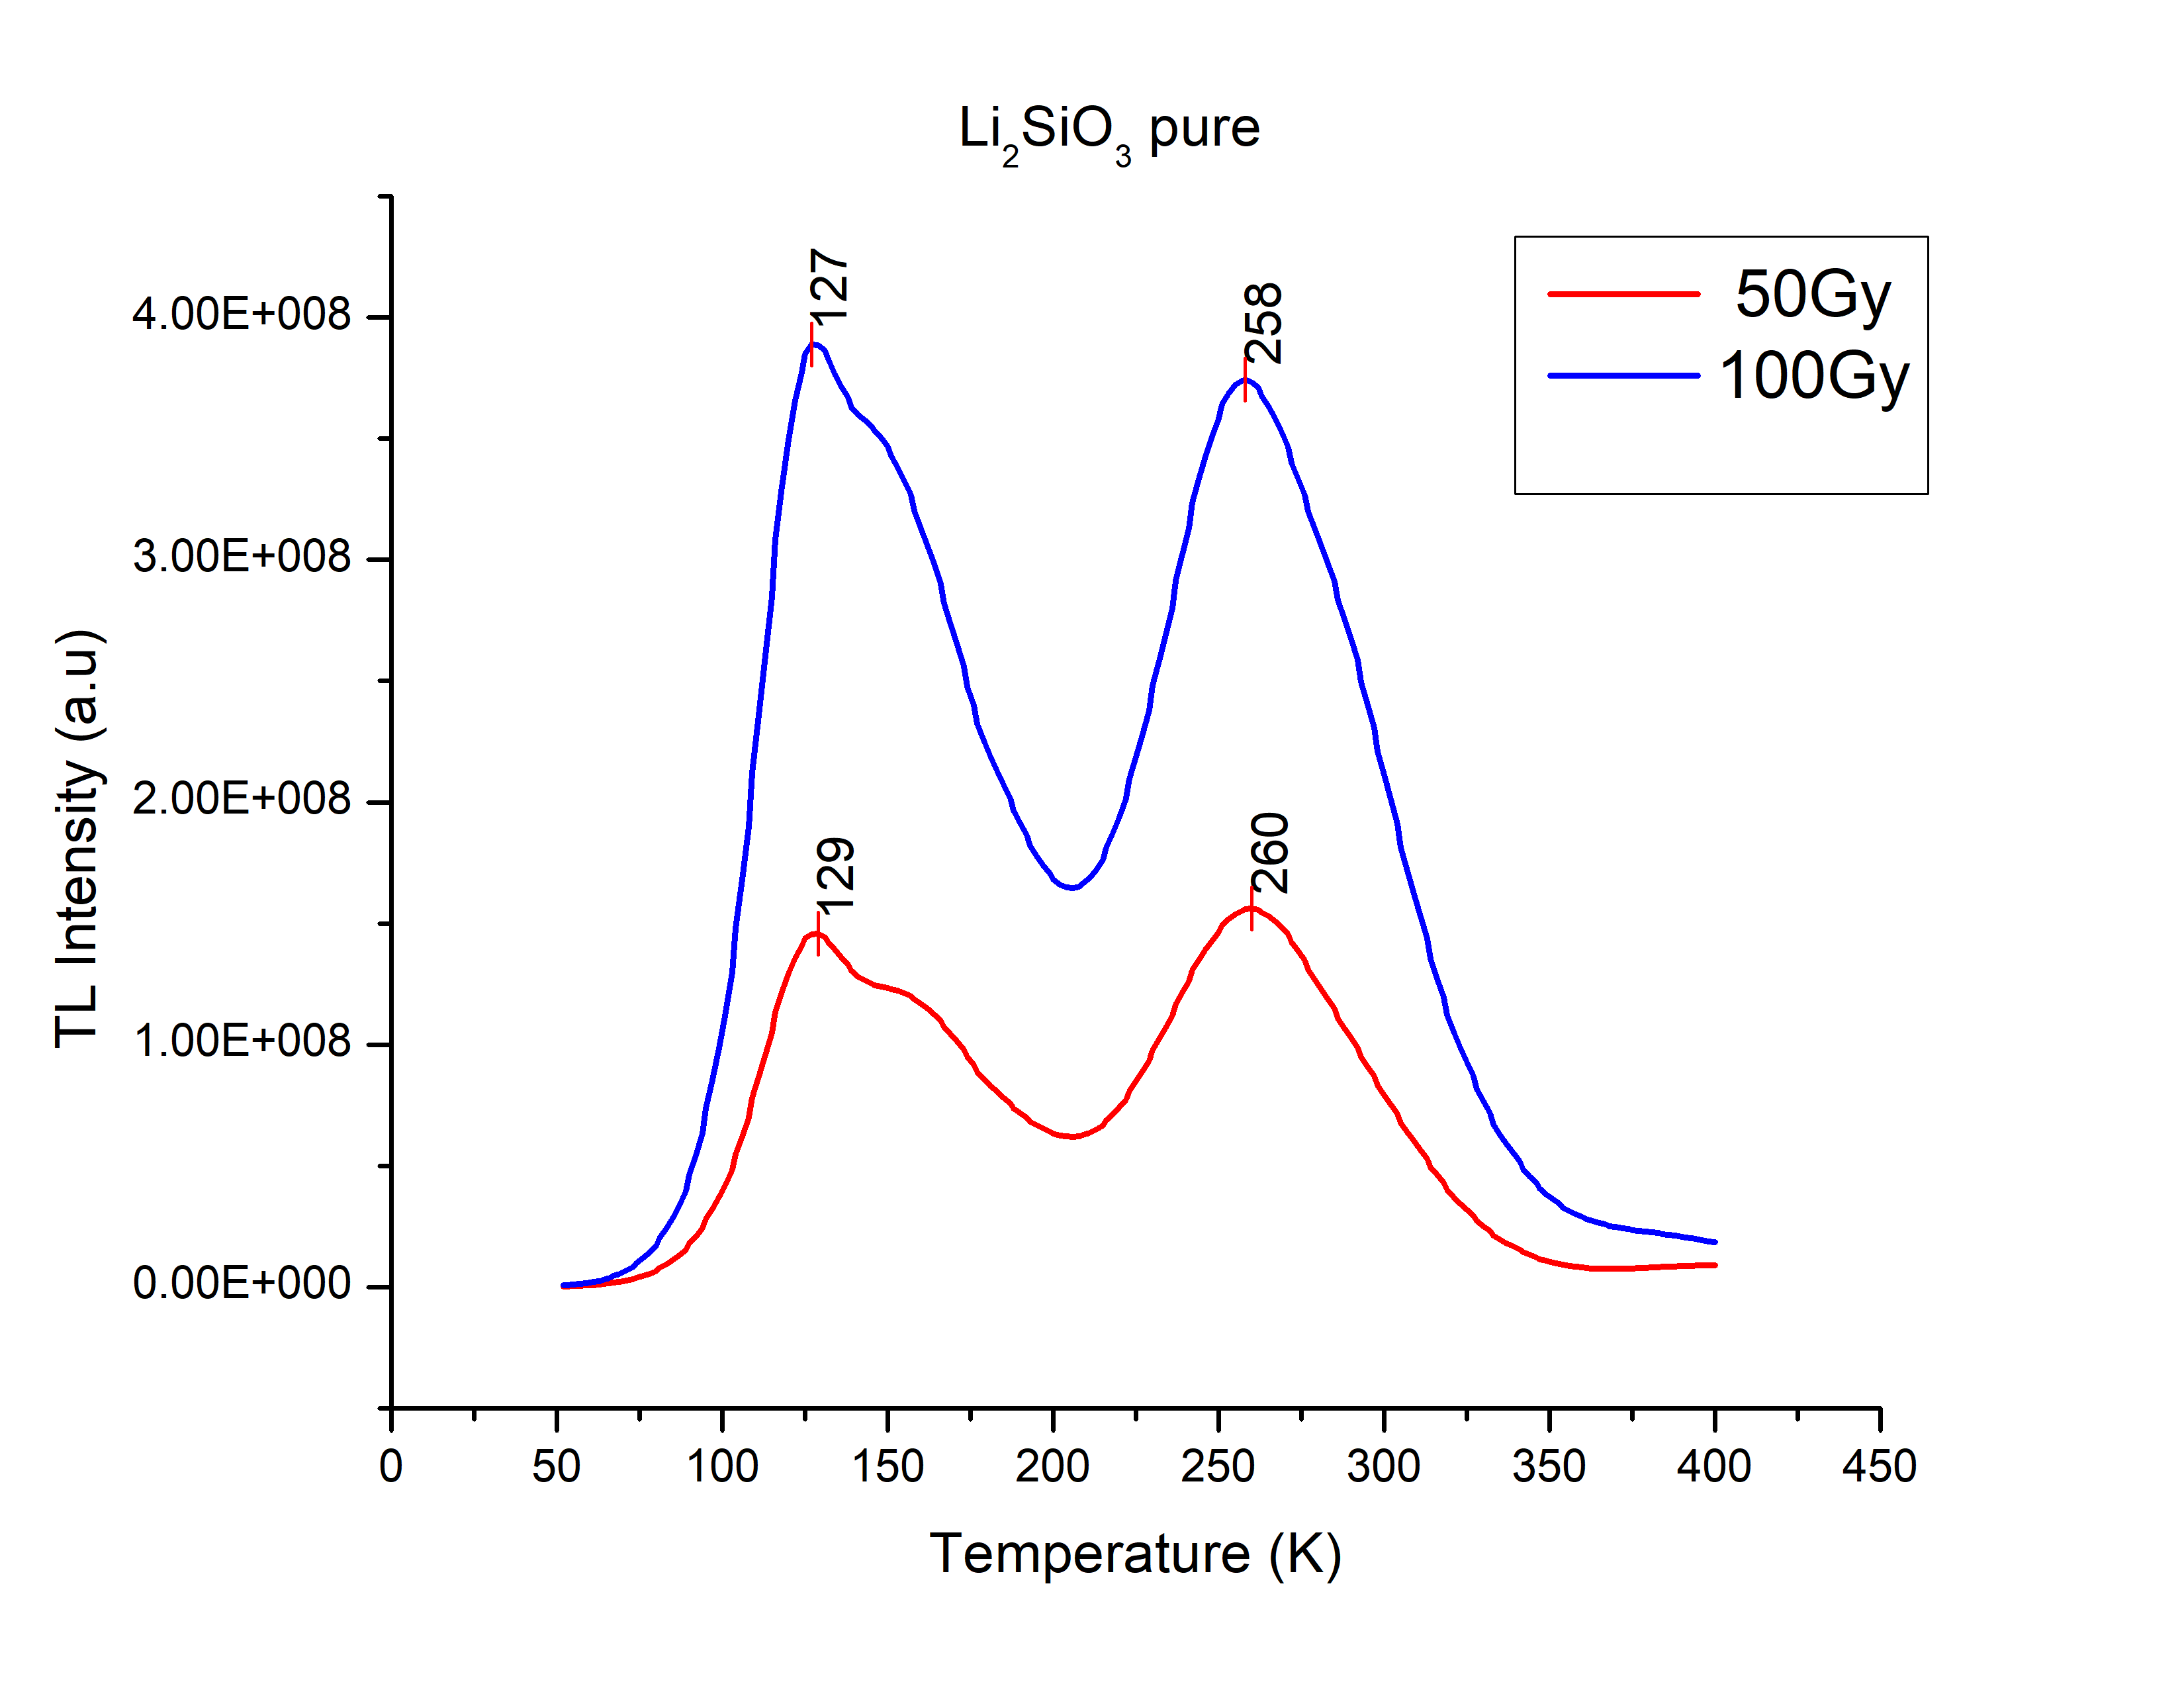
\includegraphics[width=0.8\linewidth]{lisoPure.png}
            \captionof{figure}{Dose response for Lithium metasilicate when irradiated with Gamma rays at 50 
            Gy and 100 Gy}\label{fig:lisoPure}
        \end{Figure}
        \begin{Figure}
            \centering
            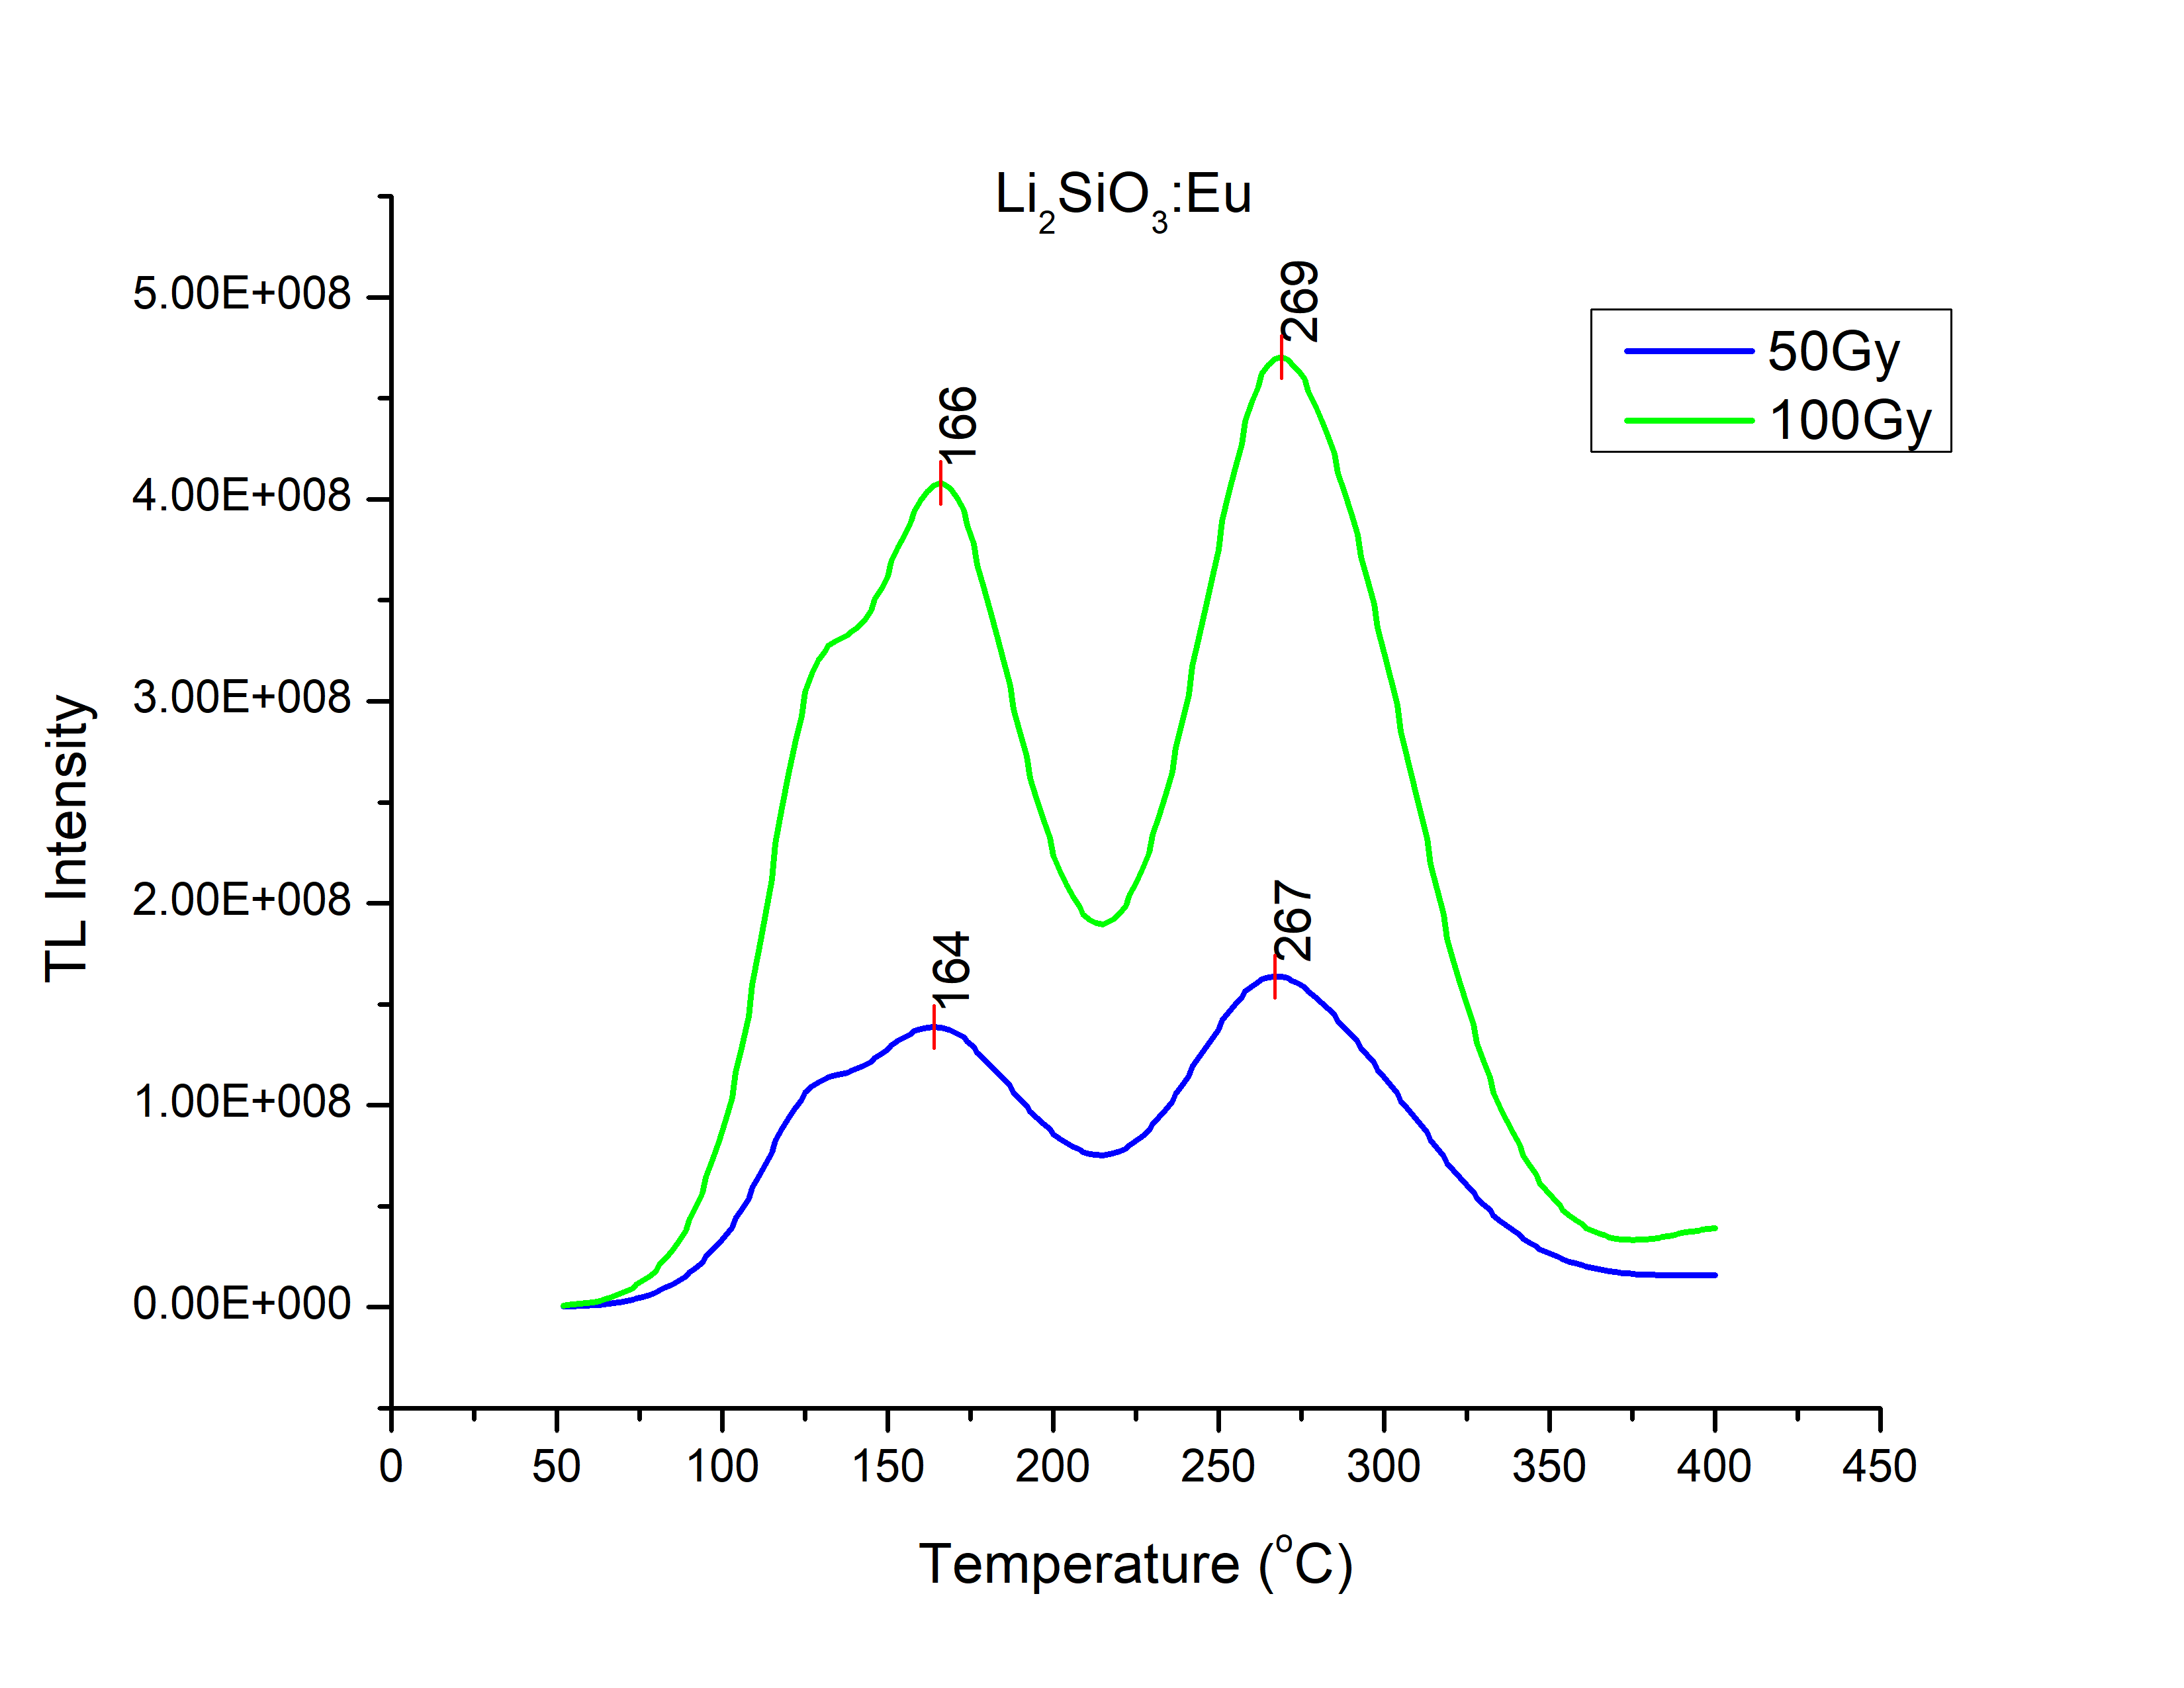
\includegraphics[width=0.8\linewidth]{lisoEu.png}
            \captionof{figure}{Dose response for Lithium metasilicate doped with 0.1mol\% Europium when irradiated 
            with Gamma rays at 50 Gy and 100 Gy}\label{fig:lisoEu}
        \end{Figure}
        \begin{Figure}
            \centering
            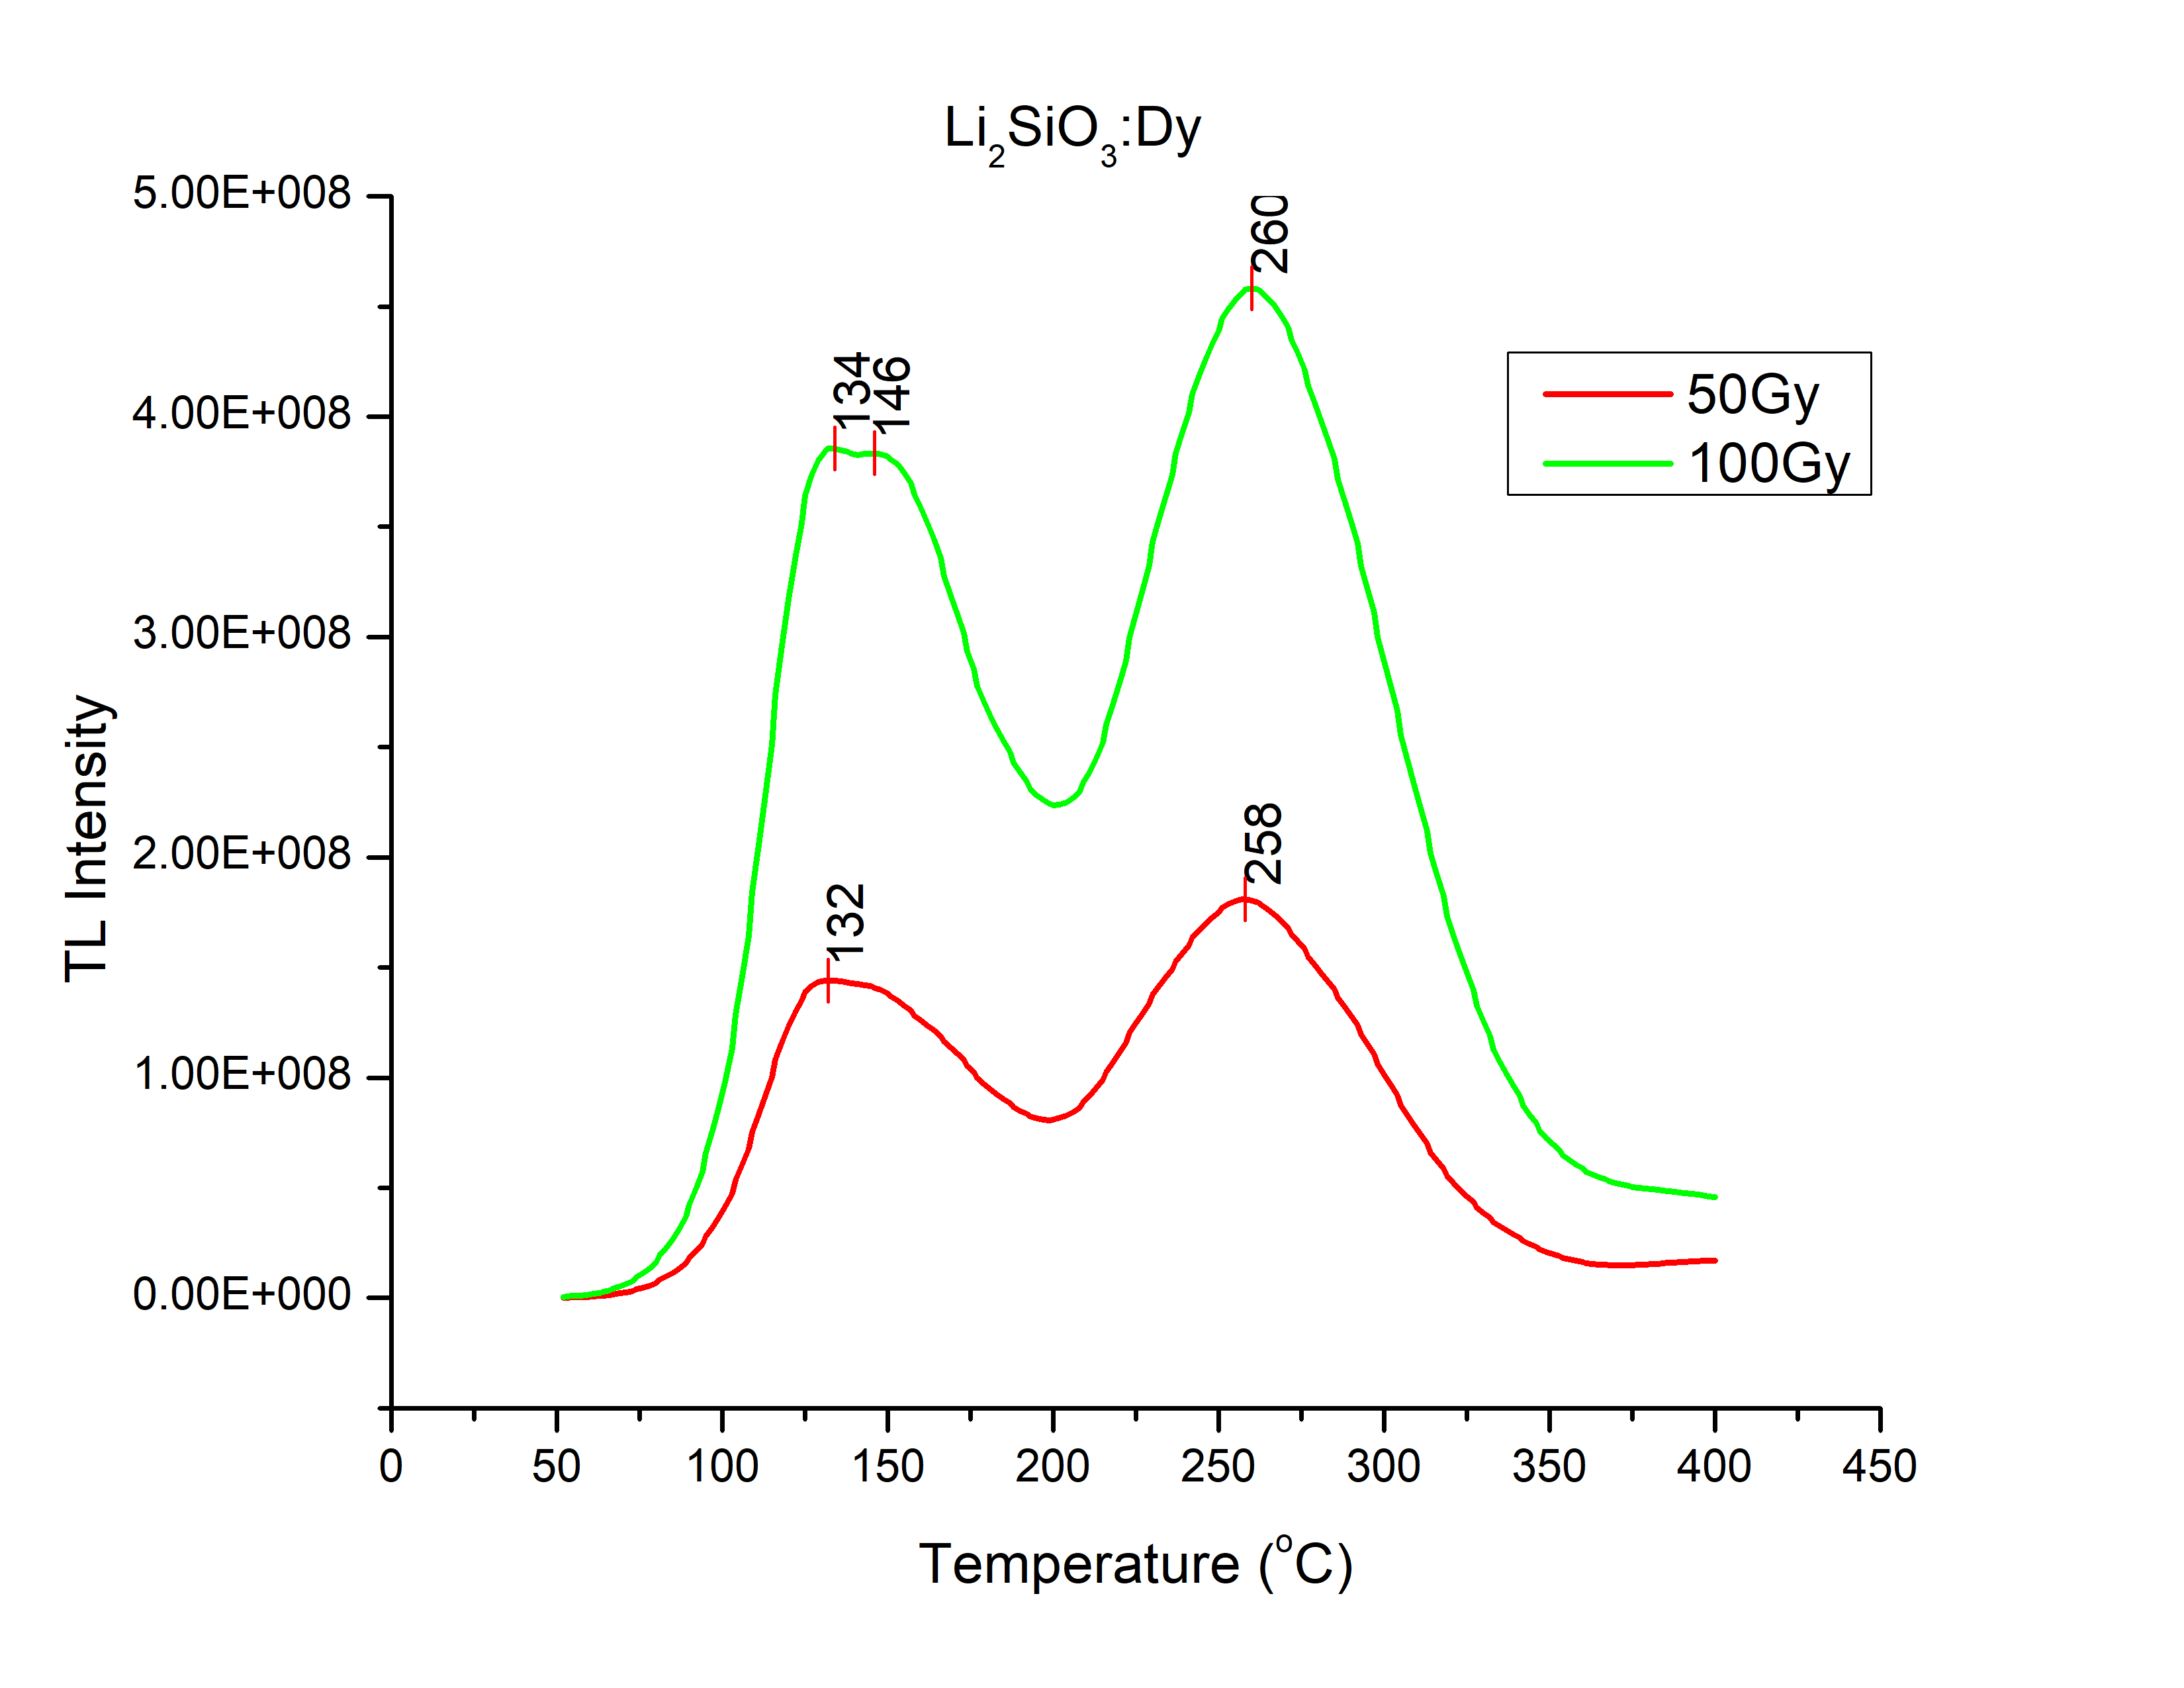
\includegraphics[width=0.8\linewidth]{lisoDy.png}
            \captionof{figure}{Dose response for Lithium metasilicate doped with 0.1mol\% Dysprosium when irradiated 
            with Gamma rays at 50 Gy and 100 Gy}\label{fig:lisoDy}
        \end{Figure}
        \begin{Figure}
            \centering
            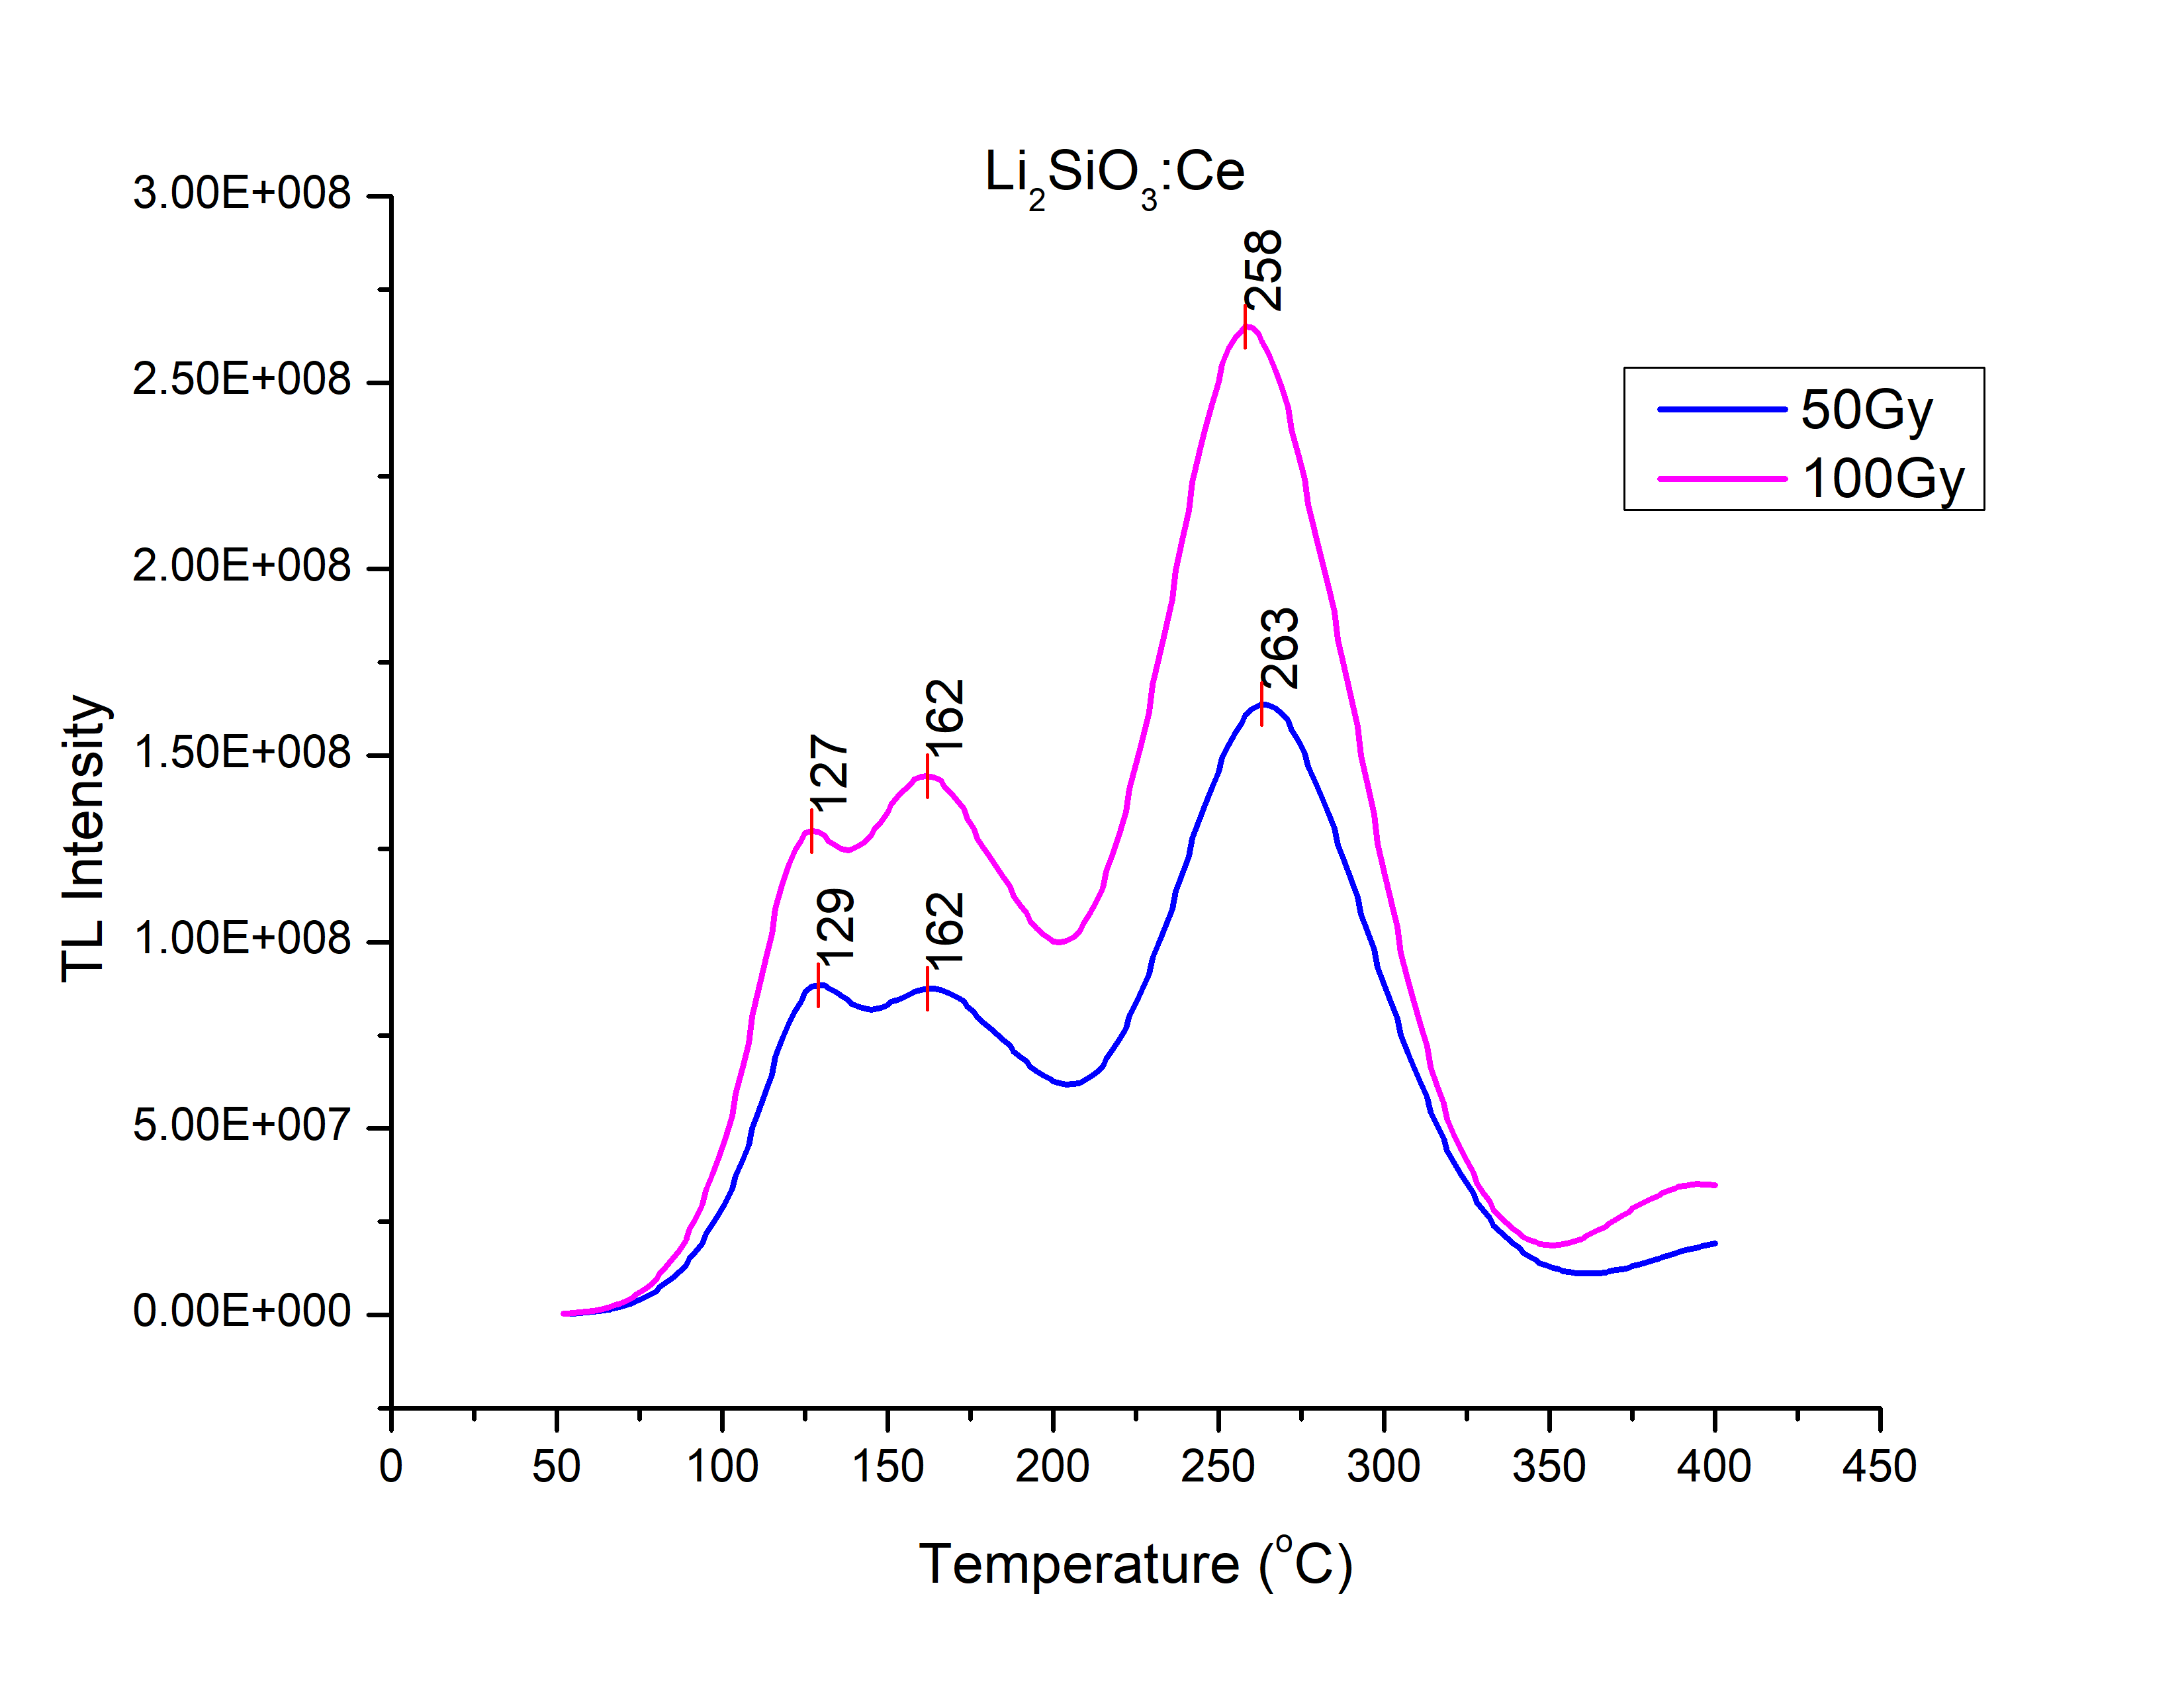
\includegraphics[width=0.8\linewidth]{lisoCe.png}
            \captionof{figure}{Dose response for Lithium metasilicate doped with 0.1mol\% Cerium when irradiated 
            with Gamma rays at 50 Gy and 100 Gy}\label{fig:lisoCe}
        \end{Figure}
        \begin{Figure}
            \centering
            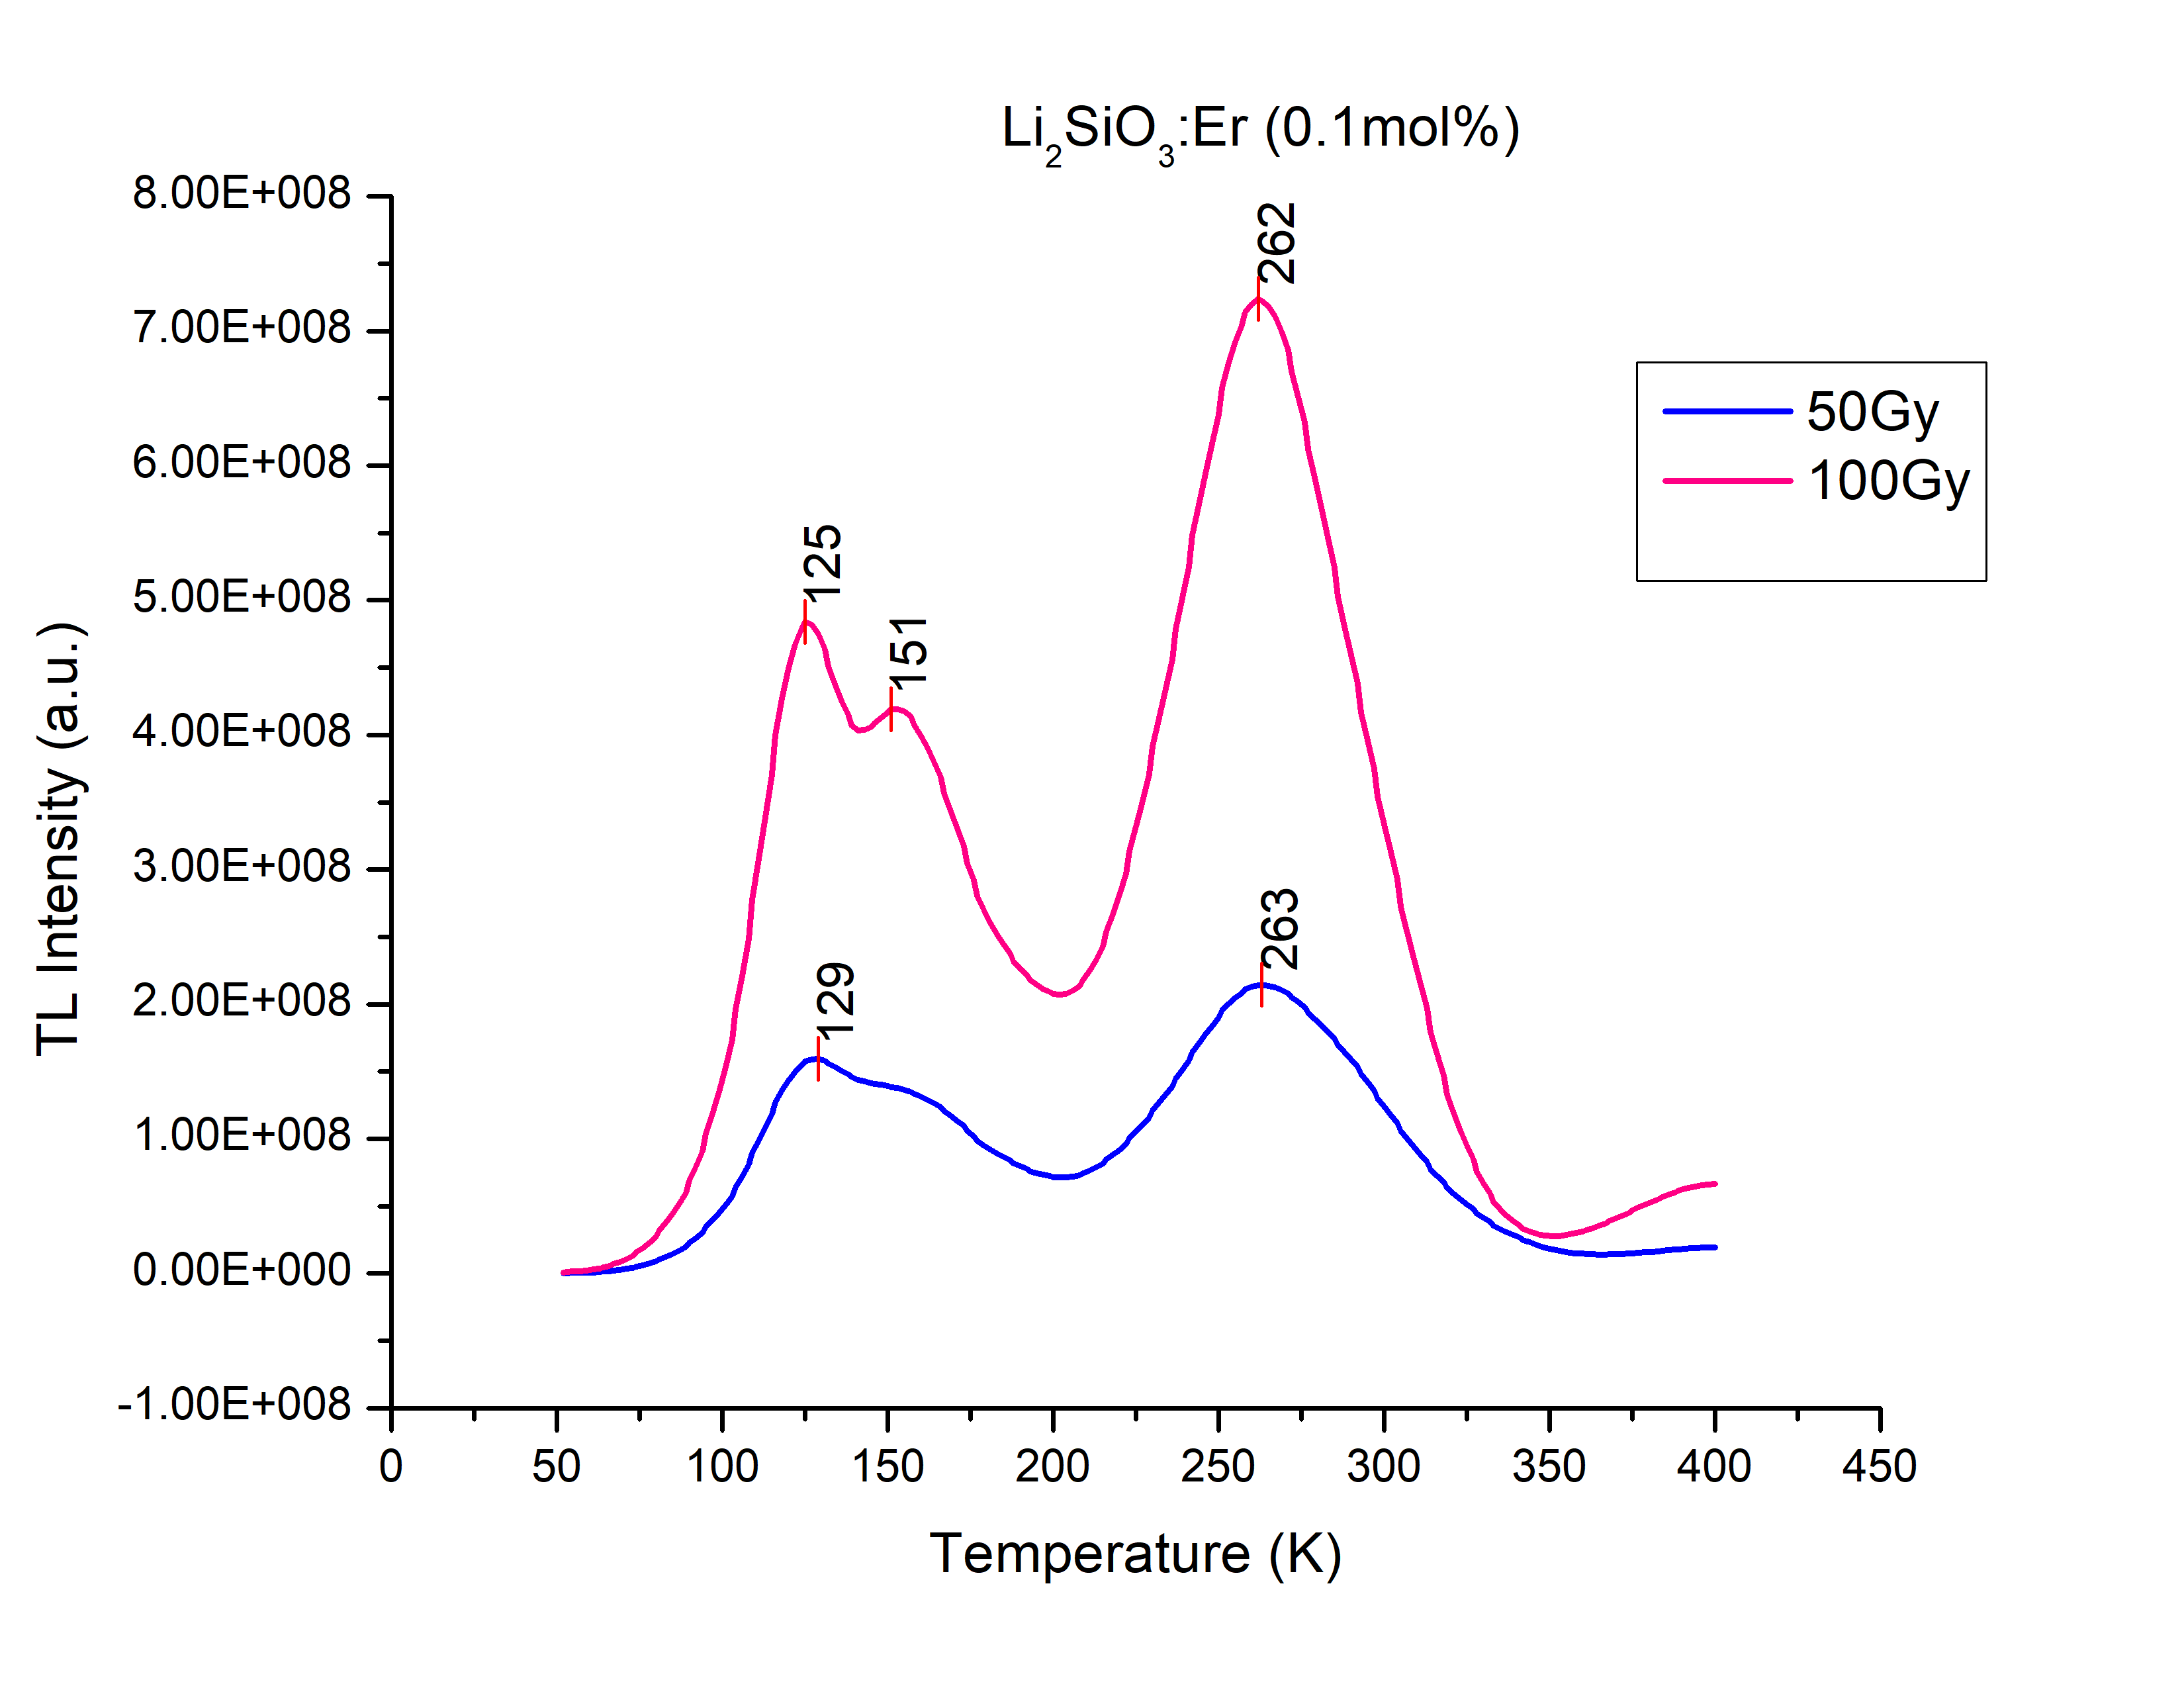
\includegraphics[width=0.8\linewidth]{lisoEr.png}
            \captionof{figure}{Dose response for Lithium metasilicate doped with 0.1mol\% Erbium when irradiated 
            with Gamma rays at 50 Gy and 100 Gy}\label{fig:lisoEr}
        \end{Figure}
        \begin{Figure}
            \centering
            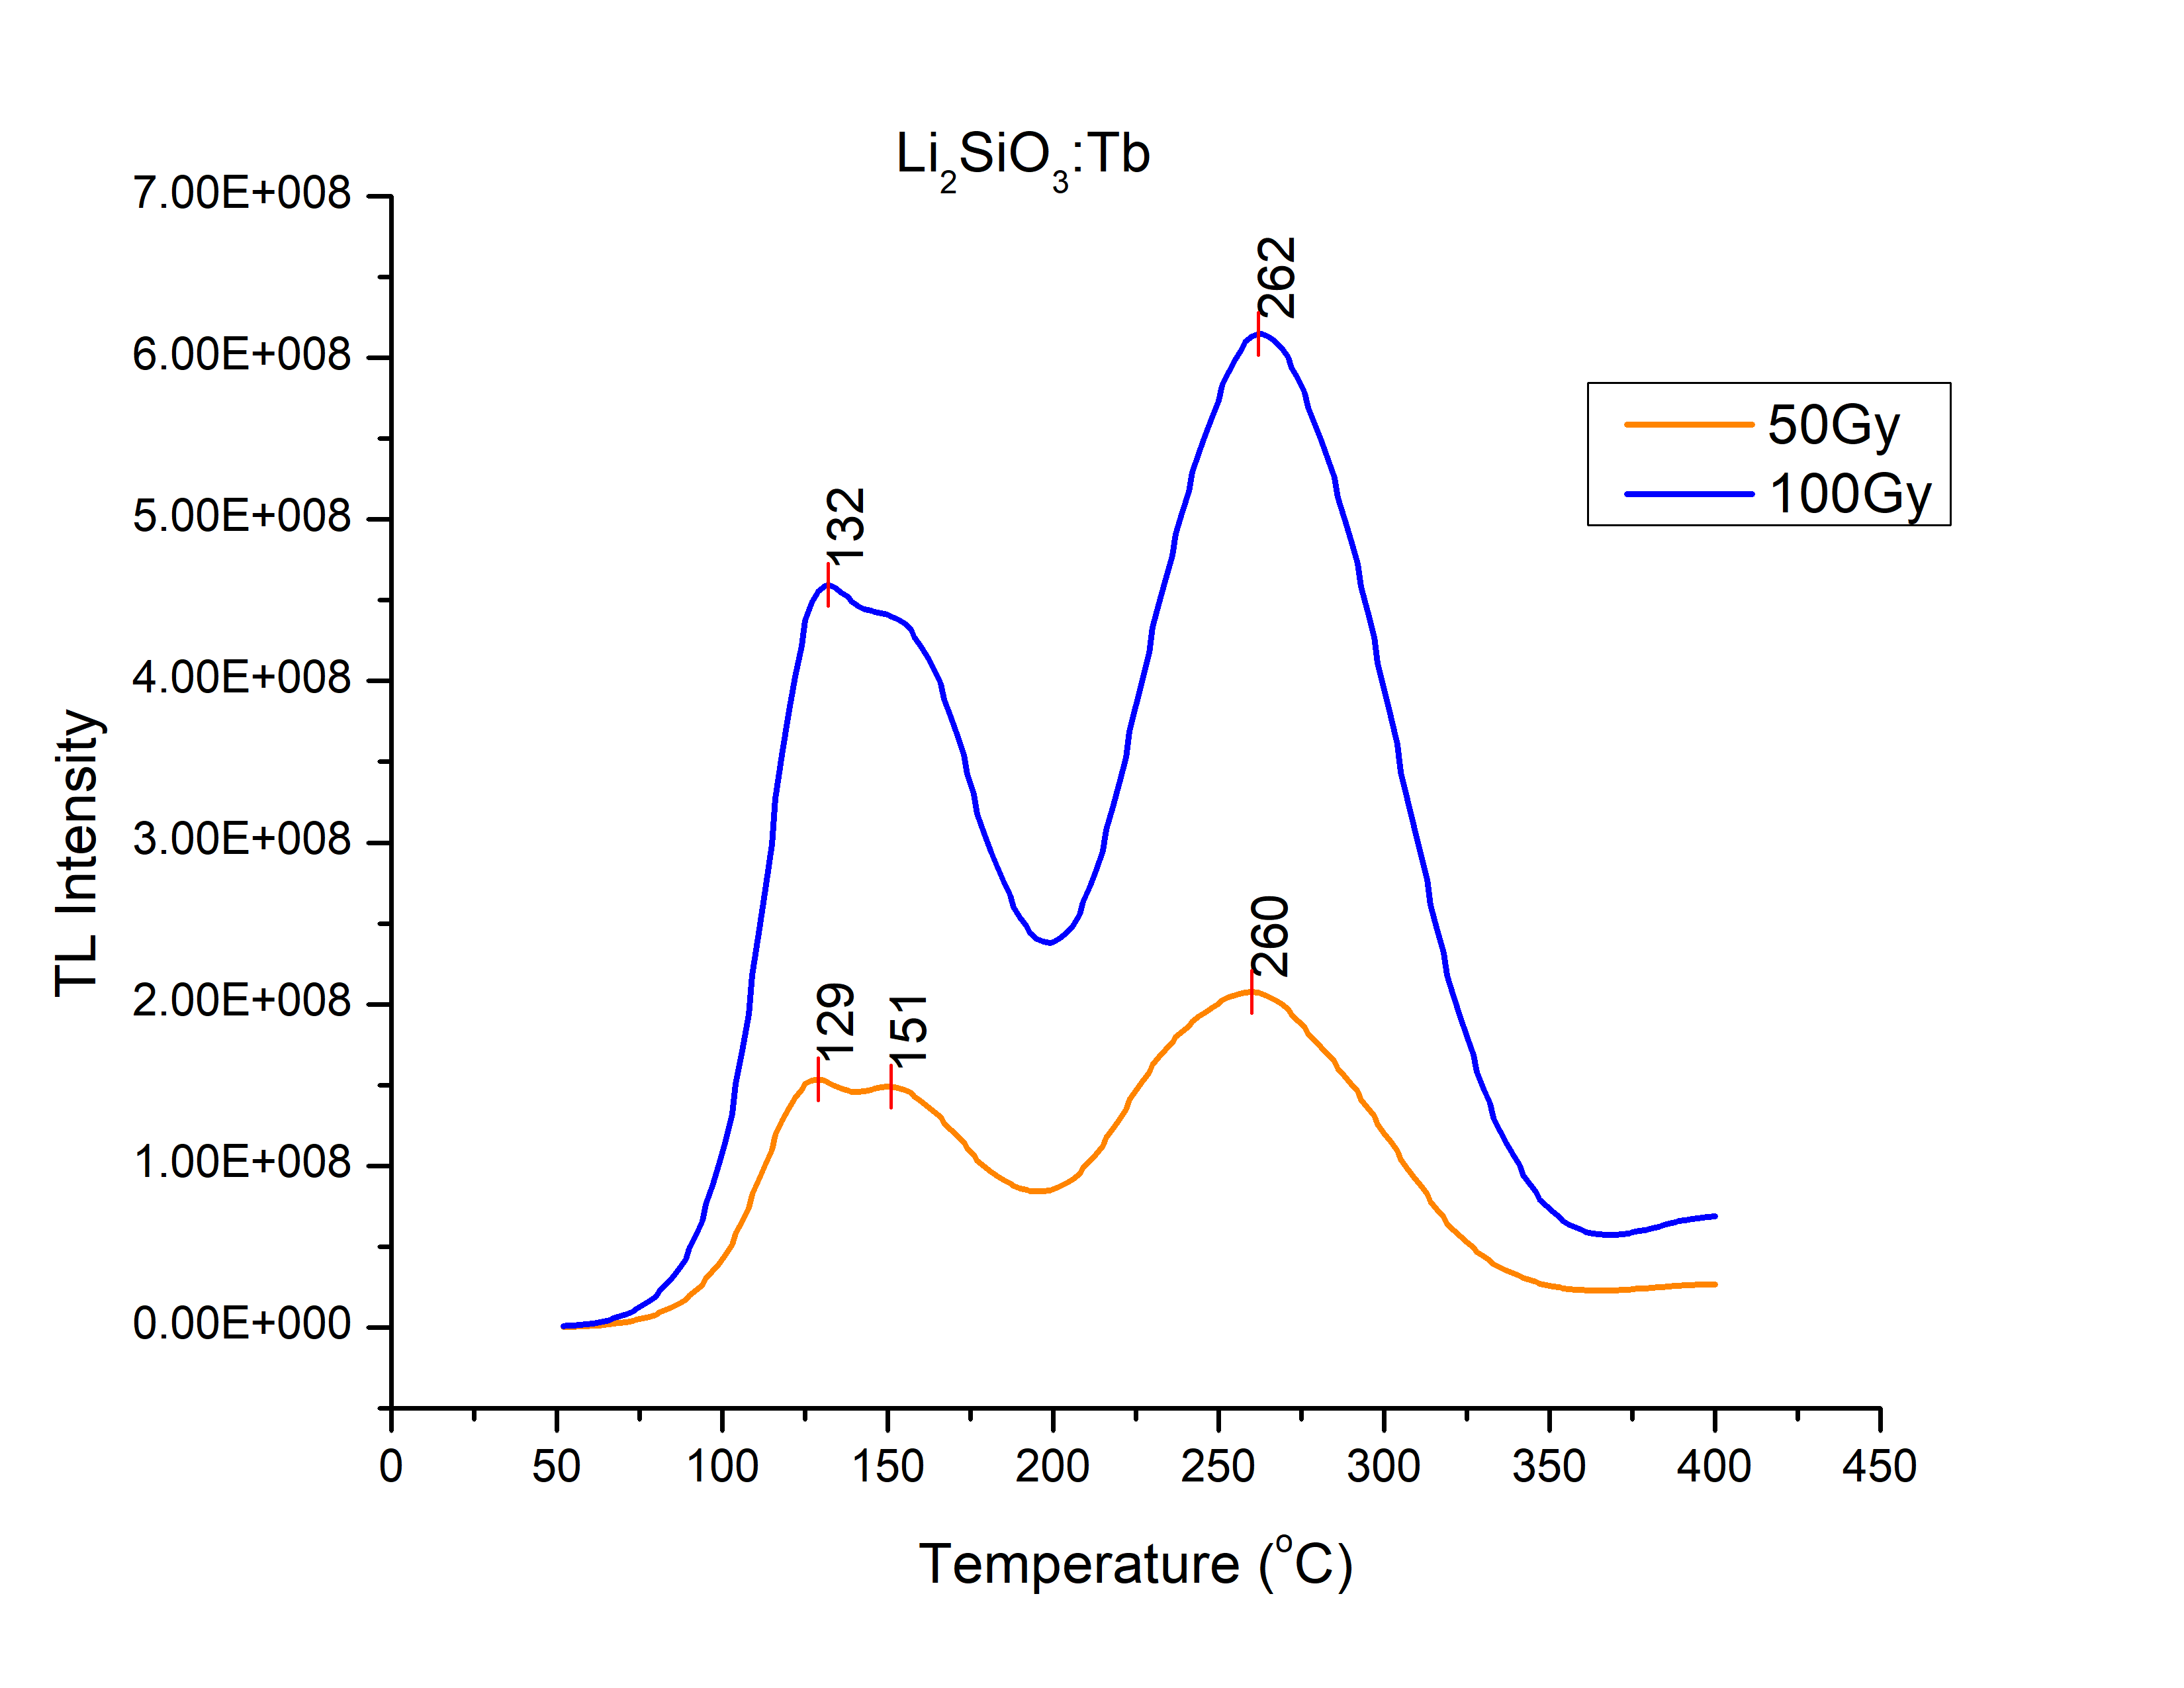
\includegraphics[width=0.8\linewidth]{lisoTb.png}
            \captionof{figure}{Dose response for Lithium metasilicate doped with 0.1mol\% Terbium when irradiated 
            with Gamma rays at 50 Gy and 100 Gy}\label{fig:lisoTb}
        \end{Figure}
    \end{multicols}
    As can be seen from the plots Lithium metasilicate yields glow curves with two to three major peaks. Pure lithium 
    metasilicate (no dopant) has peaks at $129^{\circ}C$ and $260^{\circ}C$ at 50 Gy while it peaks at $127^{\circ}C$ 
    and $258^{\circ}C$ at 100 Gy.Lithium metasilicate doped with Europium has peaks at $164^{\circ}C$ and $267^{\circ}C$ 
    at 50 Gy while at $166^{\circ}C$ and $269^{\circ}C$ at 100 Gy.Lithium metasilicate doped with Dysprosium has peaks 
    at $132^{\circ}C$ and $258^{\circ}C$ at 50 Gy while it has 3 peaks at $134^{\circ}C$,$146^{\circ}C$ and $260^{\circ}C$ 
    at 100 Gy.Lithium metasilicate doped with Cerium has 3 peaks at $129^{\circ}C$,$162^{\circ}C$ and $263^{\circ}C$ at 
    50 Gy while and at $127^{\circ}C$,$162^{\circ}C$ and $258^{\circ}C$ at 100 Gy.Lithium metasilicate doped with Erbium 
    has peaks at $129^{\circ}C$ and $263^{\circ}C$ at 50 Gy while it has 3 peaks at $125^{\circ}C$,$151^{\circ}C$ and 
    $262^{\circ}C$ at 100 Gy.Lithium metasilicate doped with Terbium has 3 peaks at $129^{\circ}C$,$151^{\circ}C$ and 
    $260^{\circ}C$ at 50 Gy while it has 2 peaks at $132^{\circ}C$ and $262^{\circ}C$ at 100 Gy.

    The effect of dopant on the dose response can be clearly seen in the following figures:
    \FloatBarrier\begin{multicols}{2}
        \begin{Figure}
            \centering
            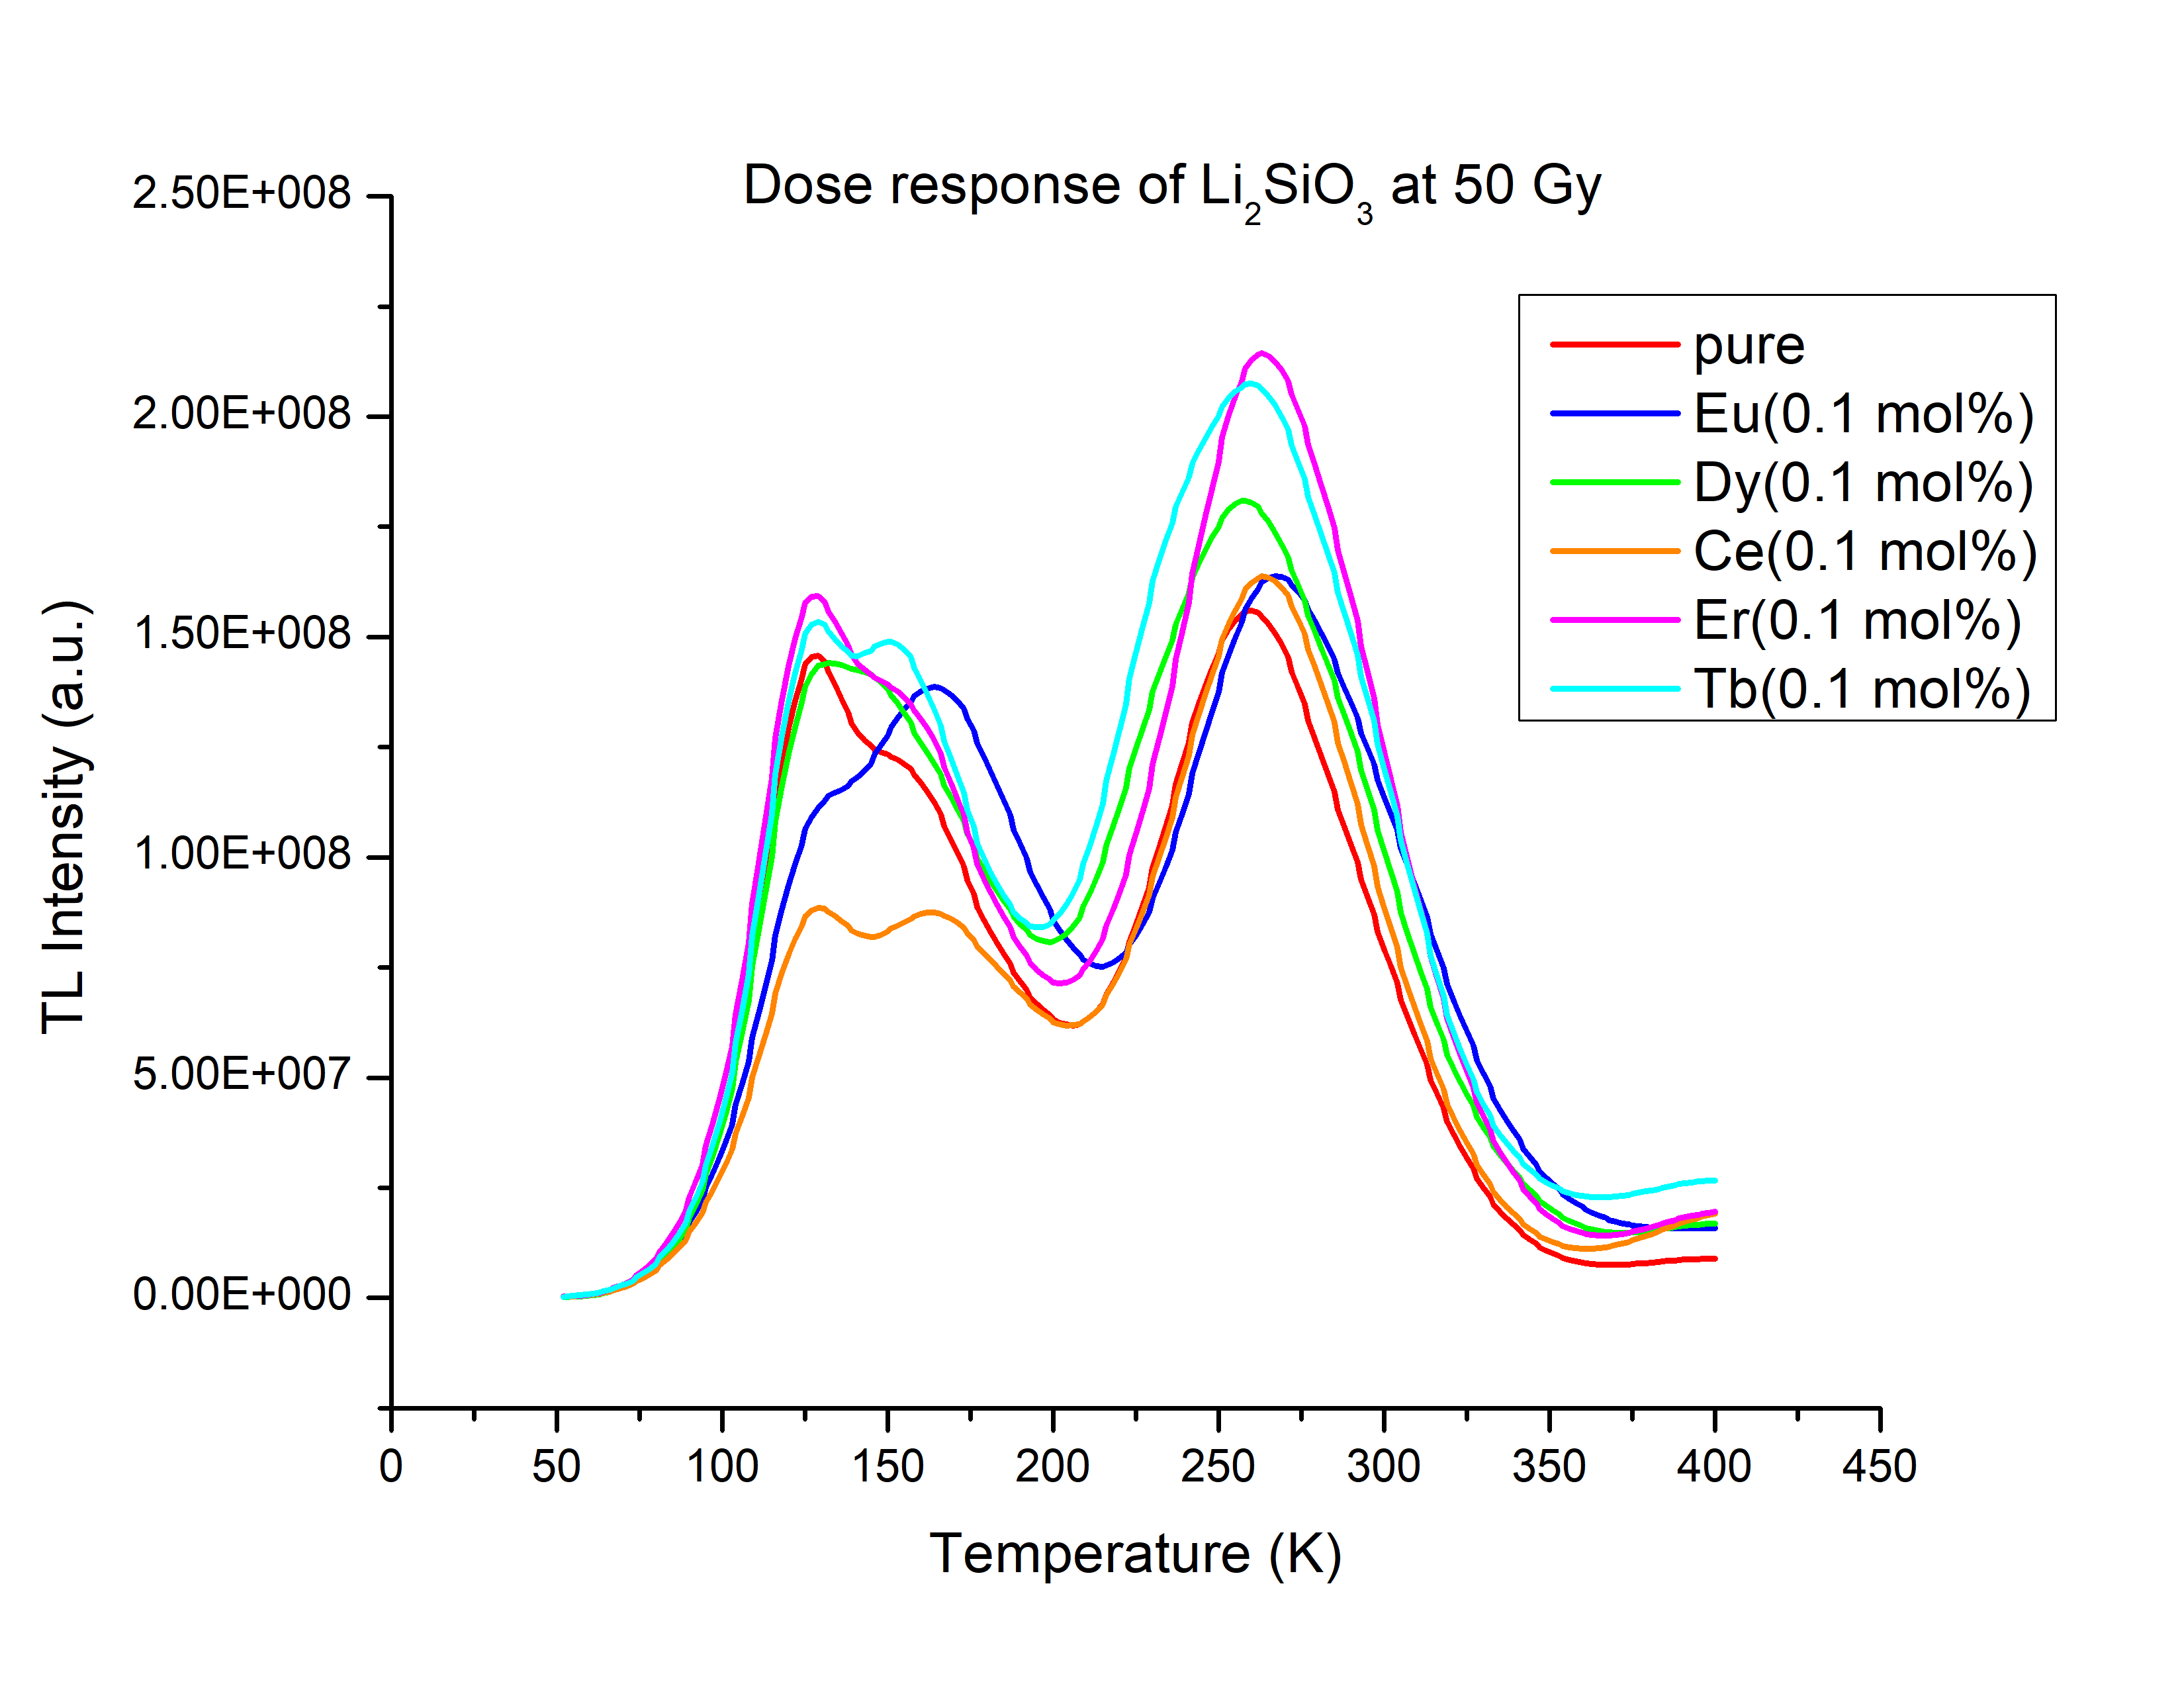
\includegraphics[width=0.8\linewidth]{tl50.png}
            \captionof{figure}{Dose response for various dopants when irradiated with Gamma rays at 50 
            Gy}\label{fig:tl50}
        \end{Figure}
        \begin{Figure}
            \centering
            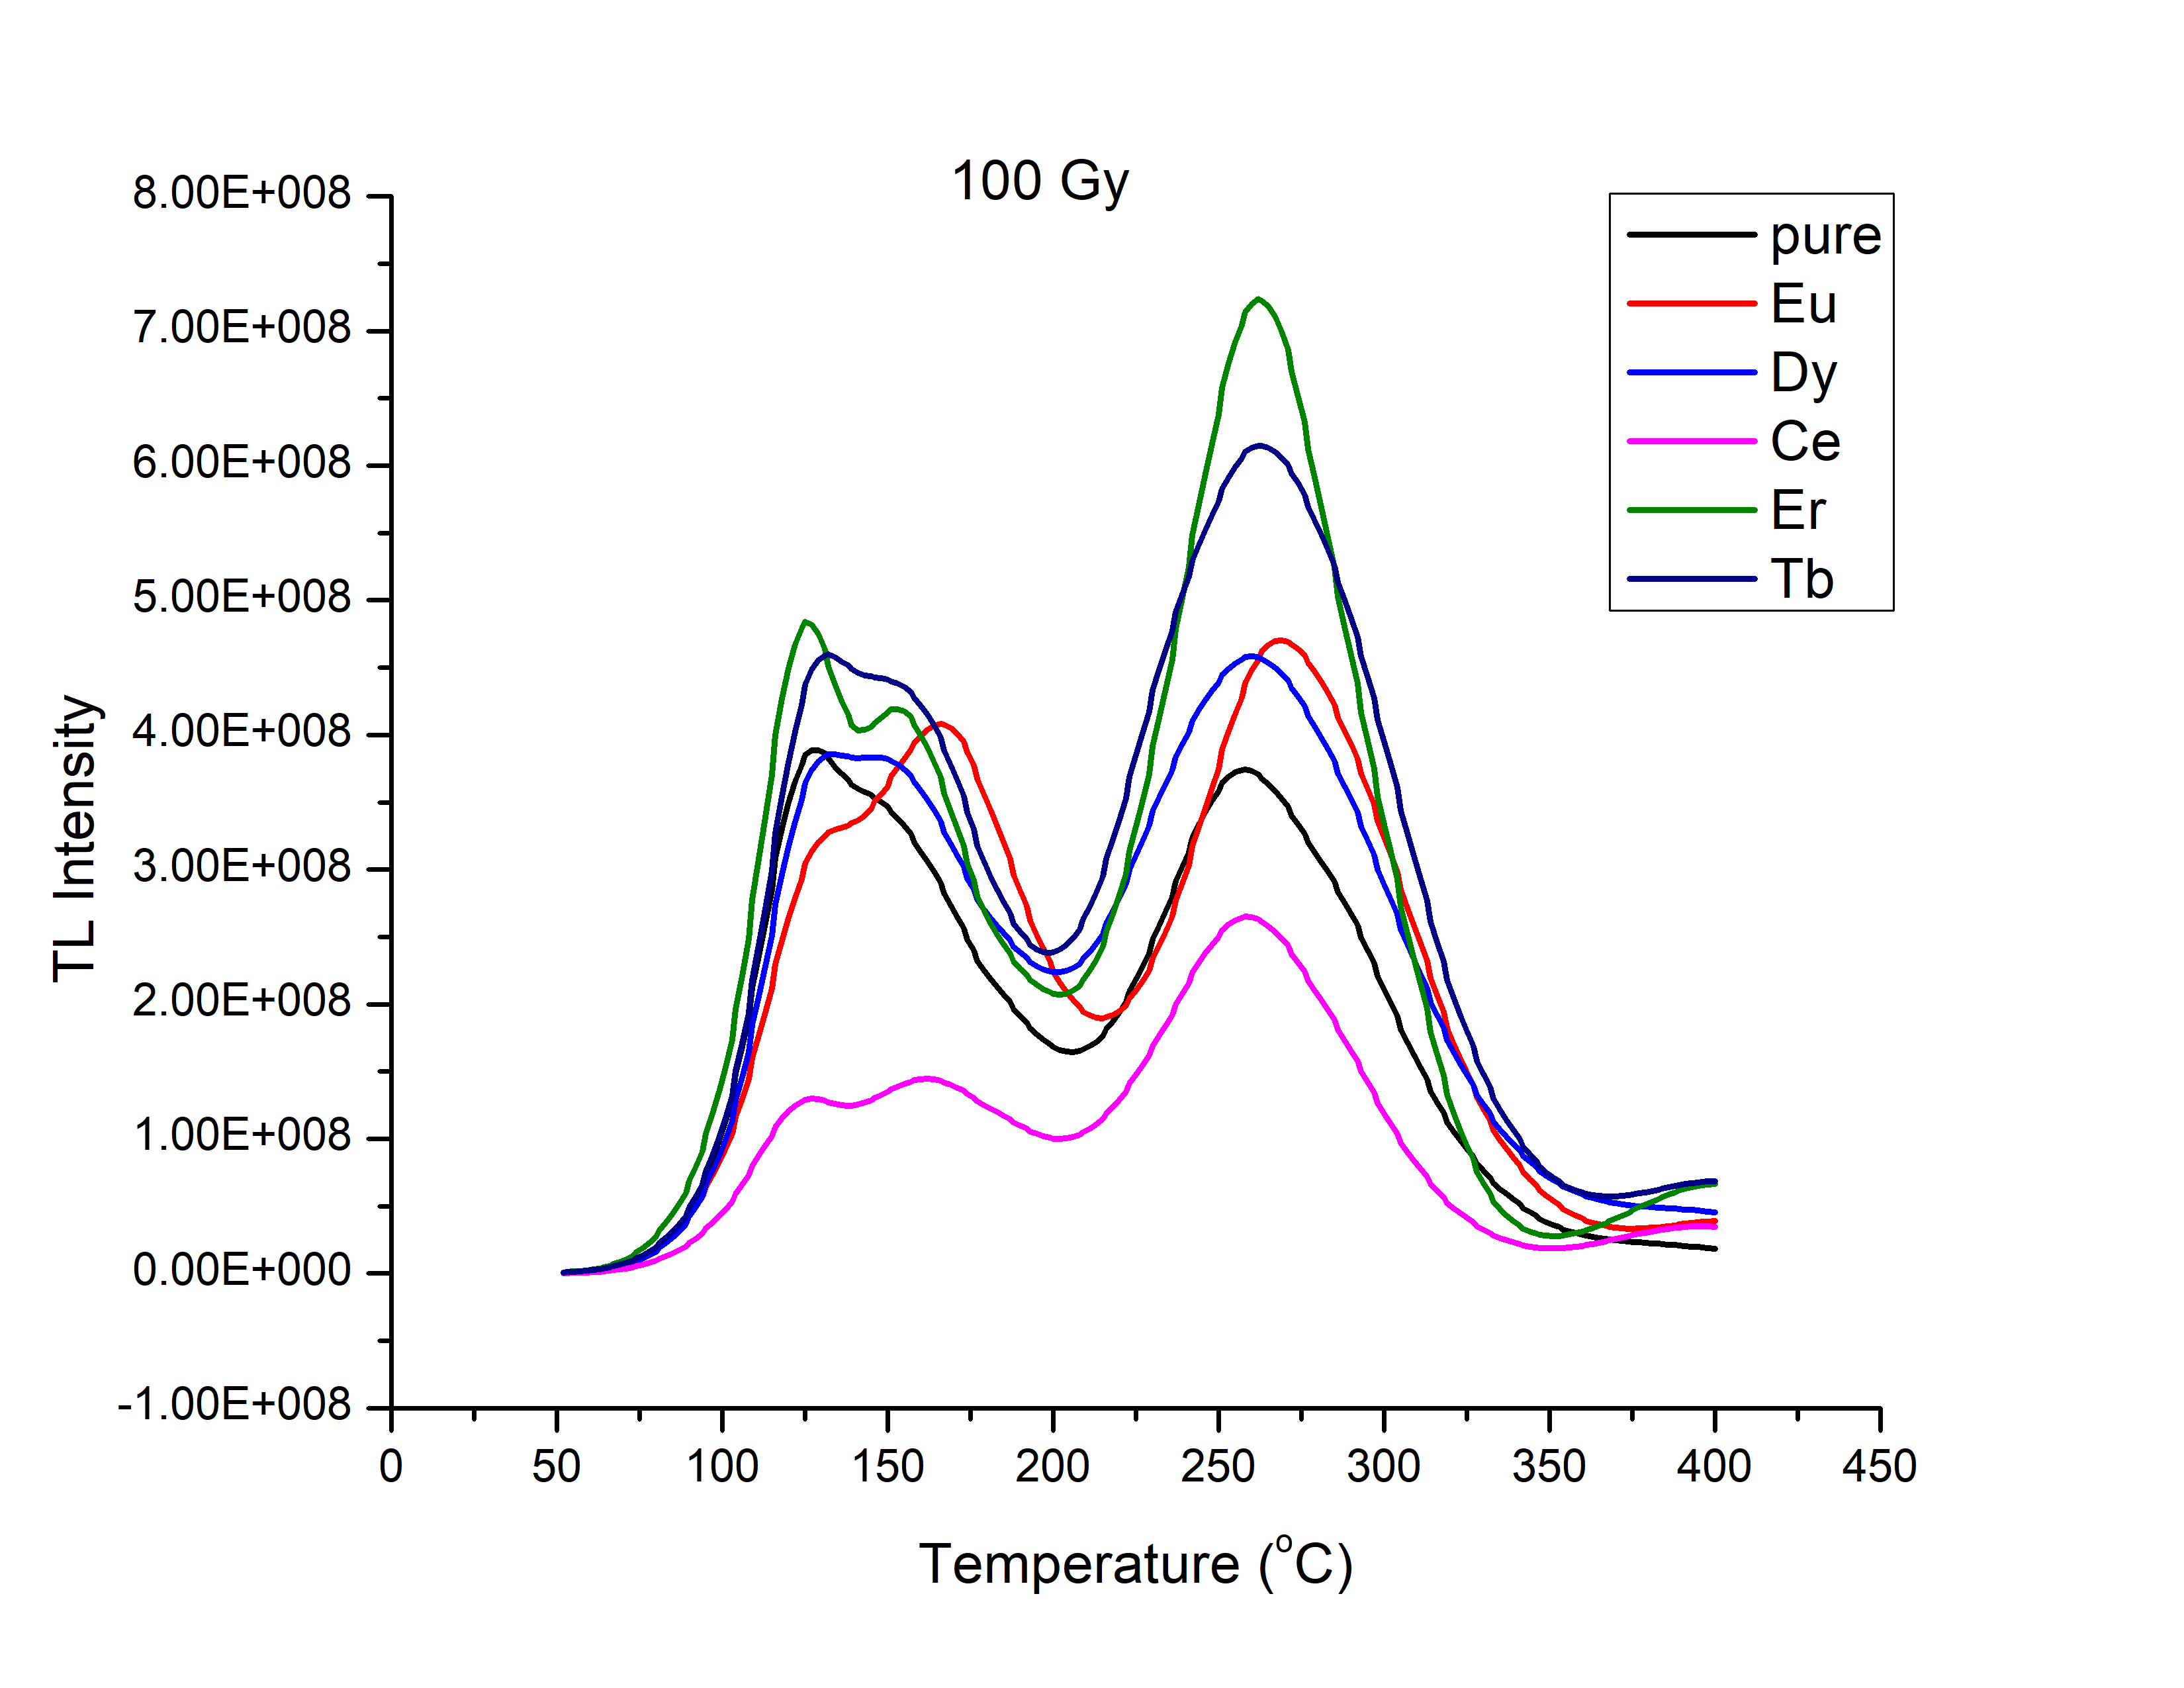
\includegraphics[width=0.8\linewidth]{tl100.png}
            \captionof{figure}{Dose response for various dopants when irradiated with Gamma rays at 100 
            Gy}\label{fig:tl100}
        \end{Figure}
    \end{multicols}

    As can be seen from the plots, doping lithium metasilicate with various dopants usually increases the thermoluminescence 
    intensity, this can be attributed to increased number of traps and recombination centres due to doping. Maximum 
    increase in intensity was observed after doping with Terbium and Erbium. A comparision plot is given below:

    \FloatBarrier\begin{multicols}{2}
        \begin{Figure}
            \centering
            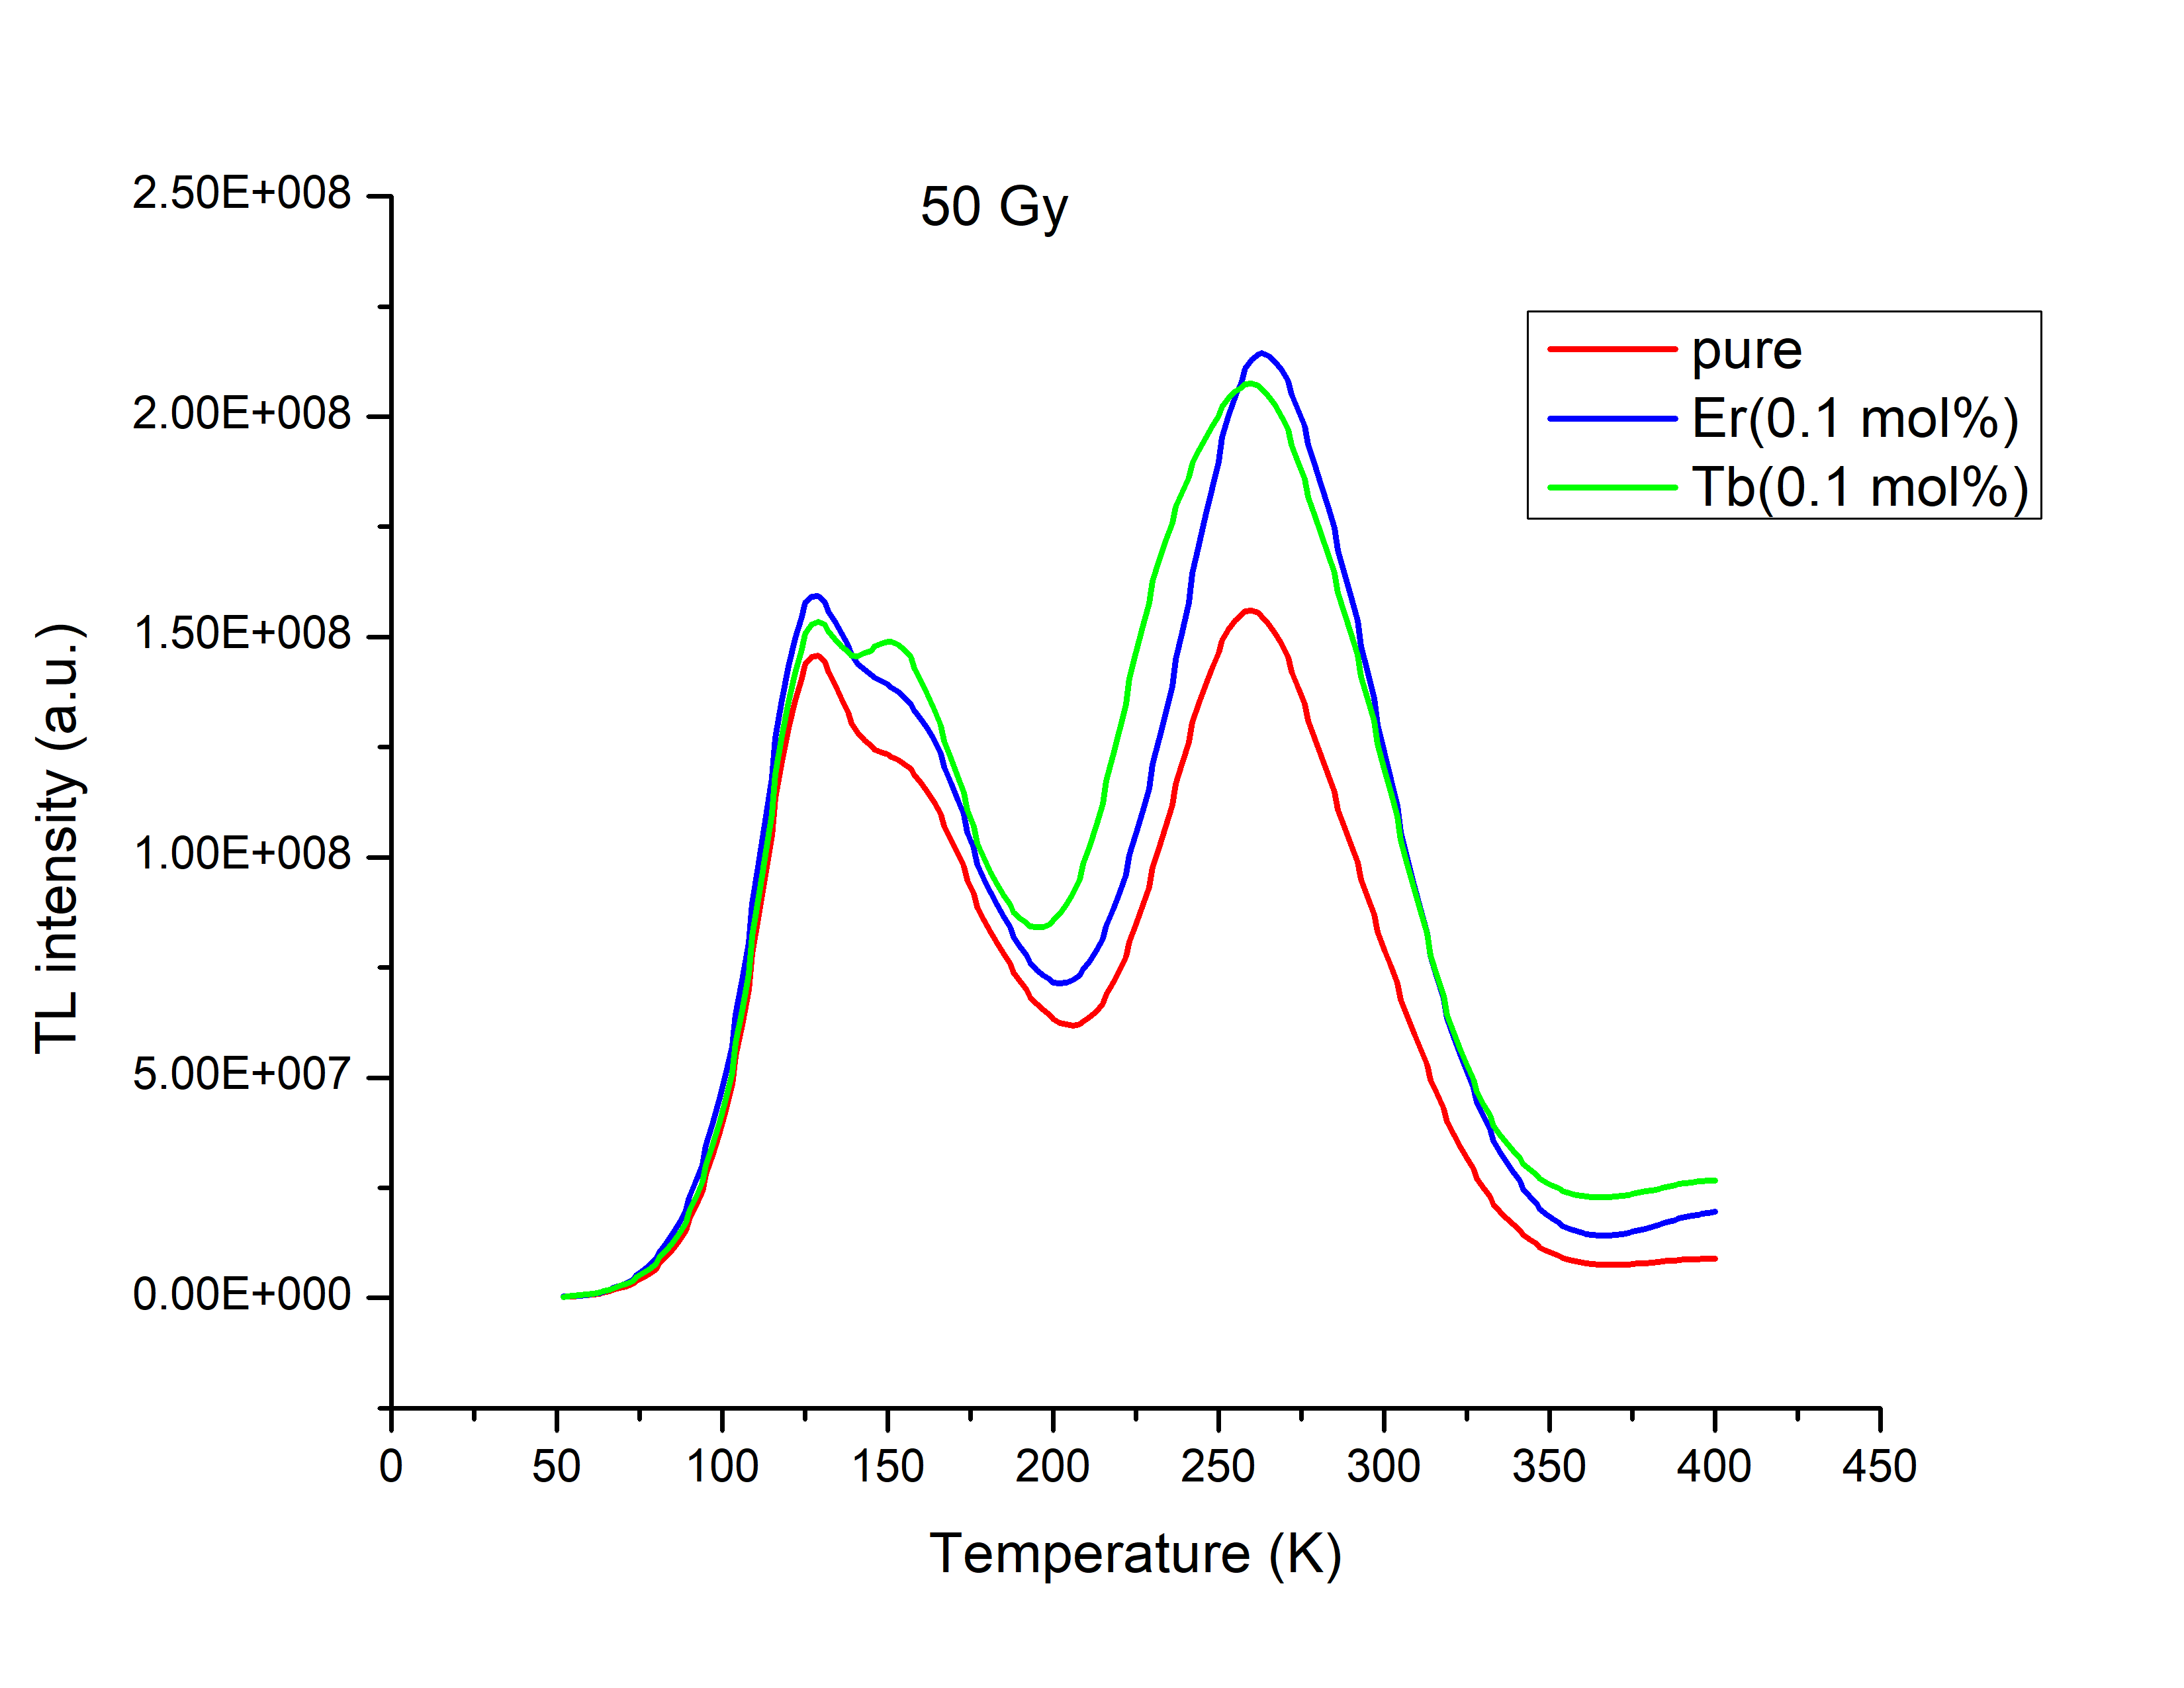
\includegraphics[width=0.8\linewidth]{comp50.png}
            \captionof{figure}{Comparision of dose response of $Li_2SiO_3$ without doping and after doping with
            Terbium and Erbium when irradiated with Gamma rays at 50 Gy}\label{fig:comp50}
        \end{Figure}
        \begin{Figure}
            \centering
            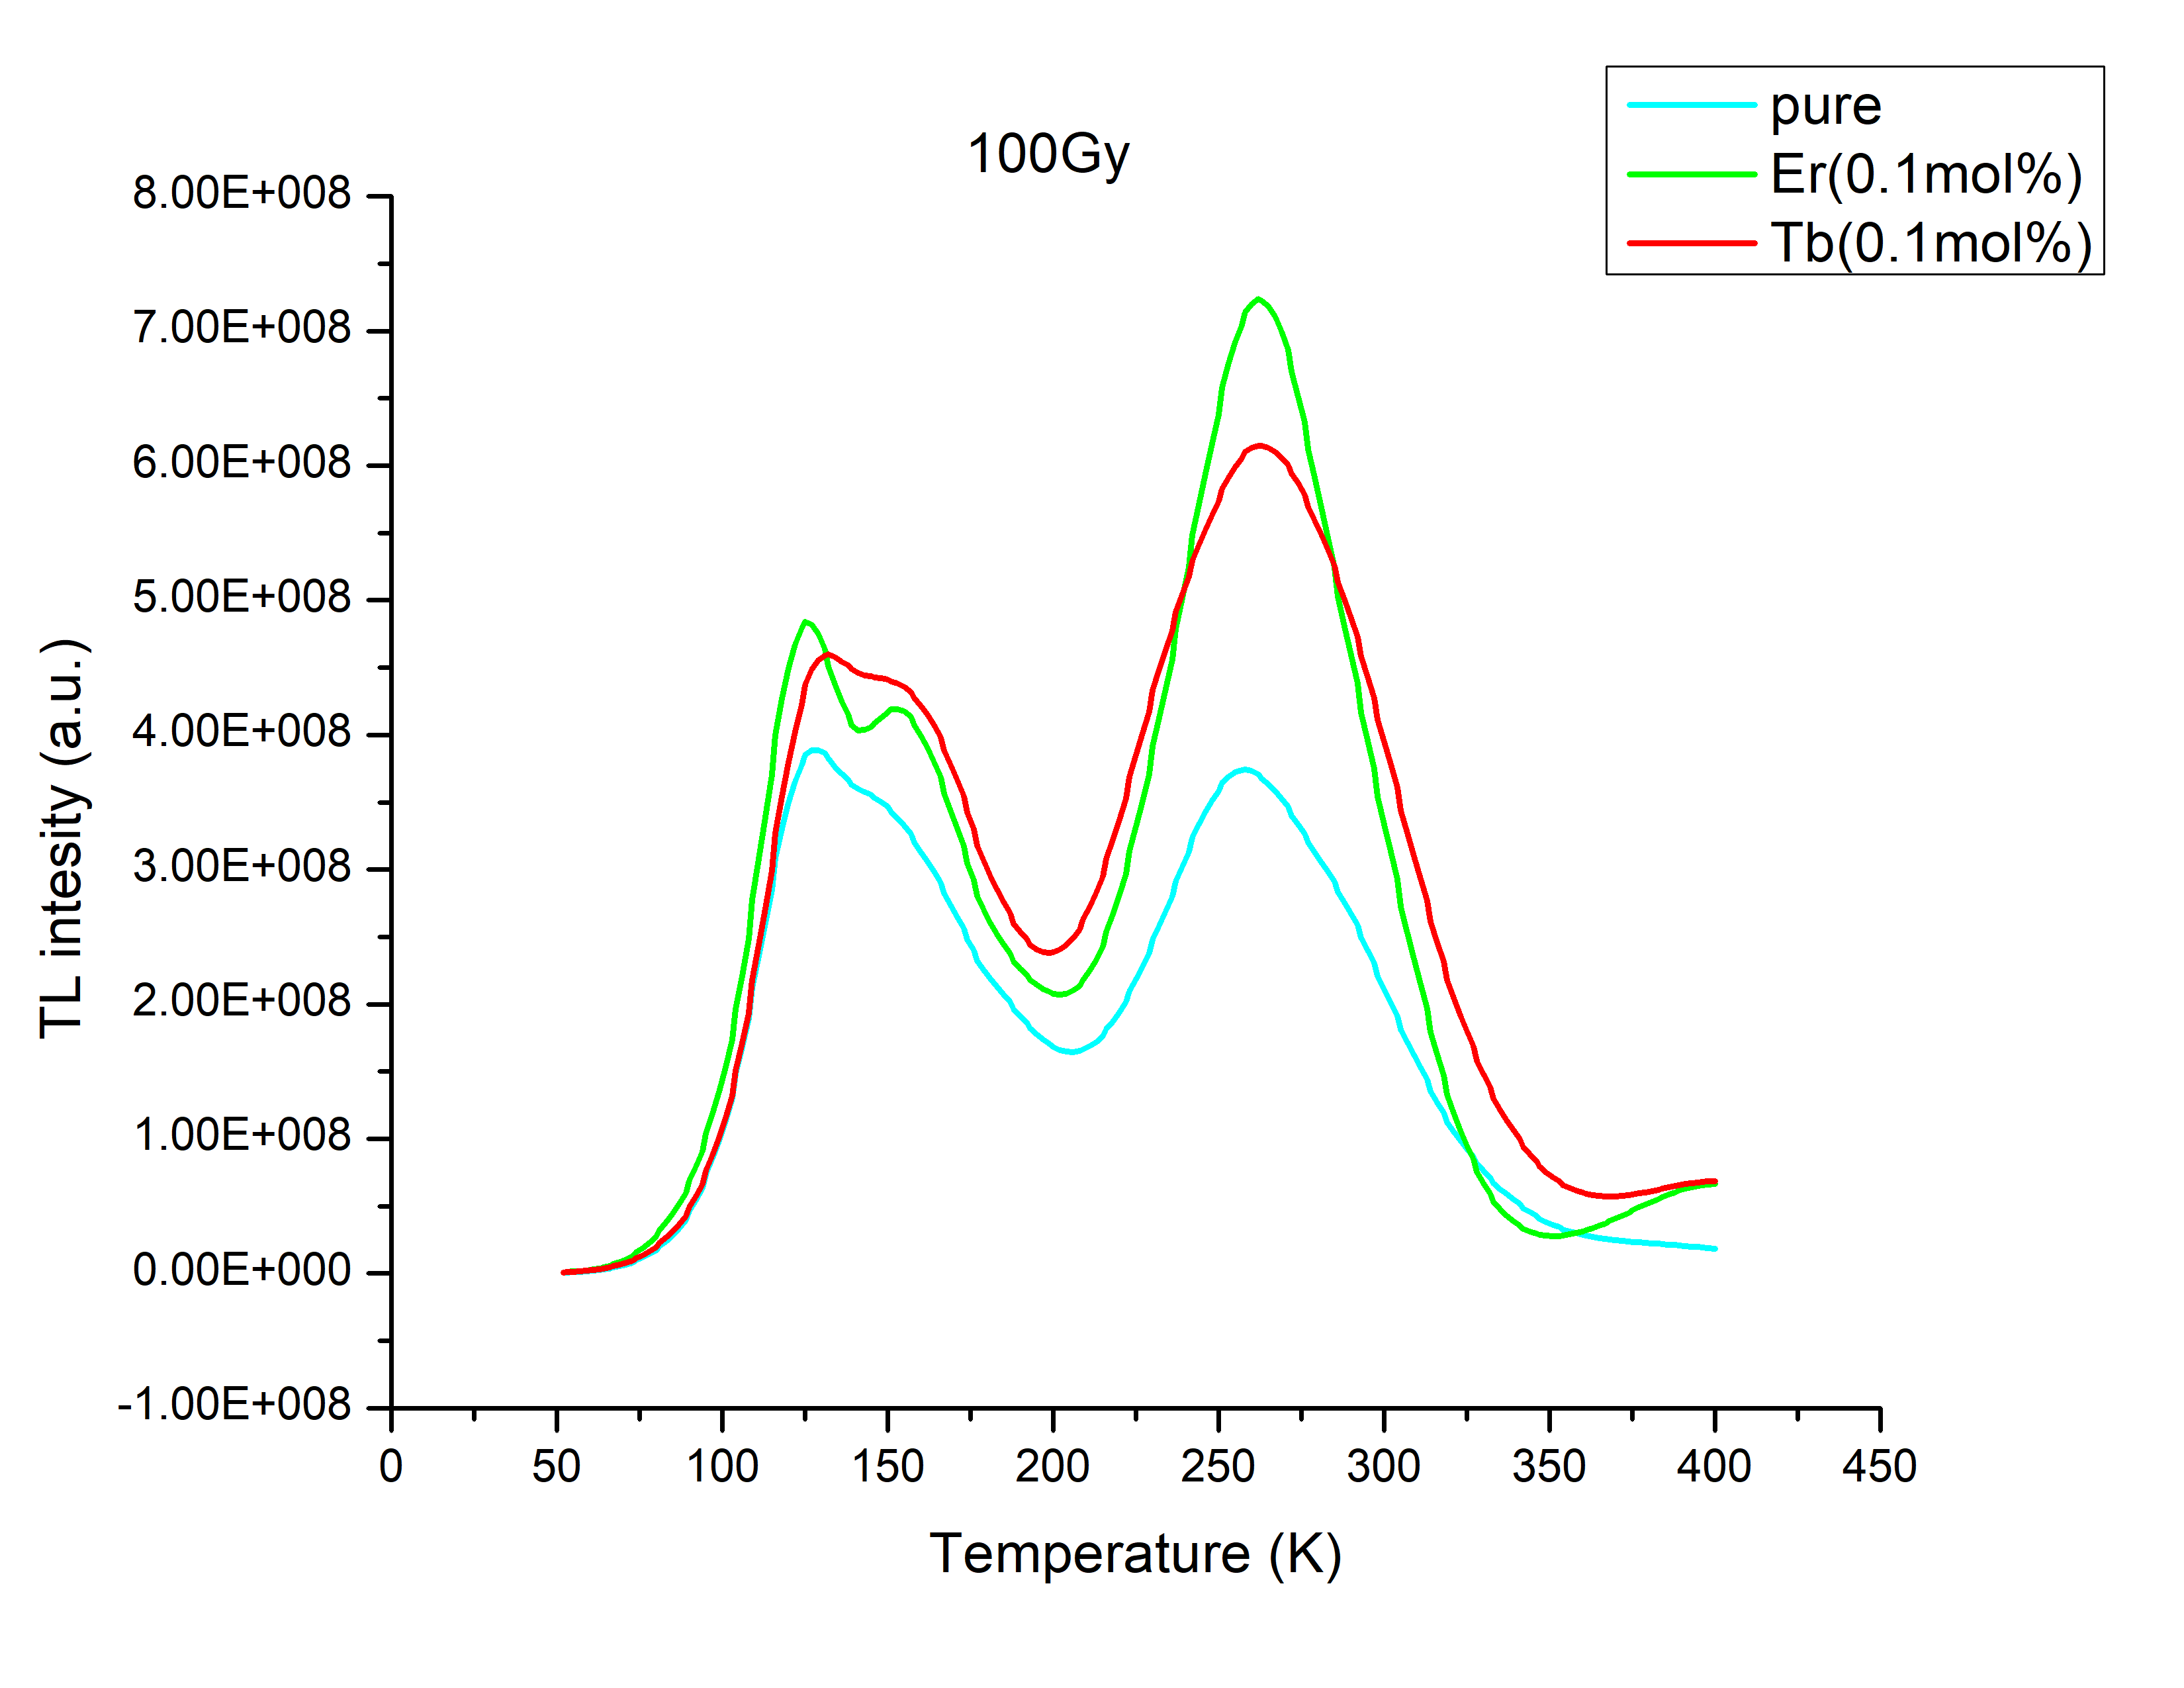
\includegraphics[width=0.8\linewidth]{comp100.png}
            \captionof{figure}{Comparision of dose response of $Li_2SiO_3$ without doping and after doping with
            Terbium and Erbium when irradiated with Gamma rays at 100 Gy}\label{fig:comp100}
        \end{Figure}
    \end{multicols}

    A comparision between peak intensities has been done for various dopants at both 50 Gy and 100 gy gamma ray 
    irradiation. These plots indicate that the peak intensity for Terbium and Erbium is much higher as compared to 
    other dopants. 

    \FloatBarrier\begin{multicols}{2}
        \begin{Figure}
            \centering
            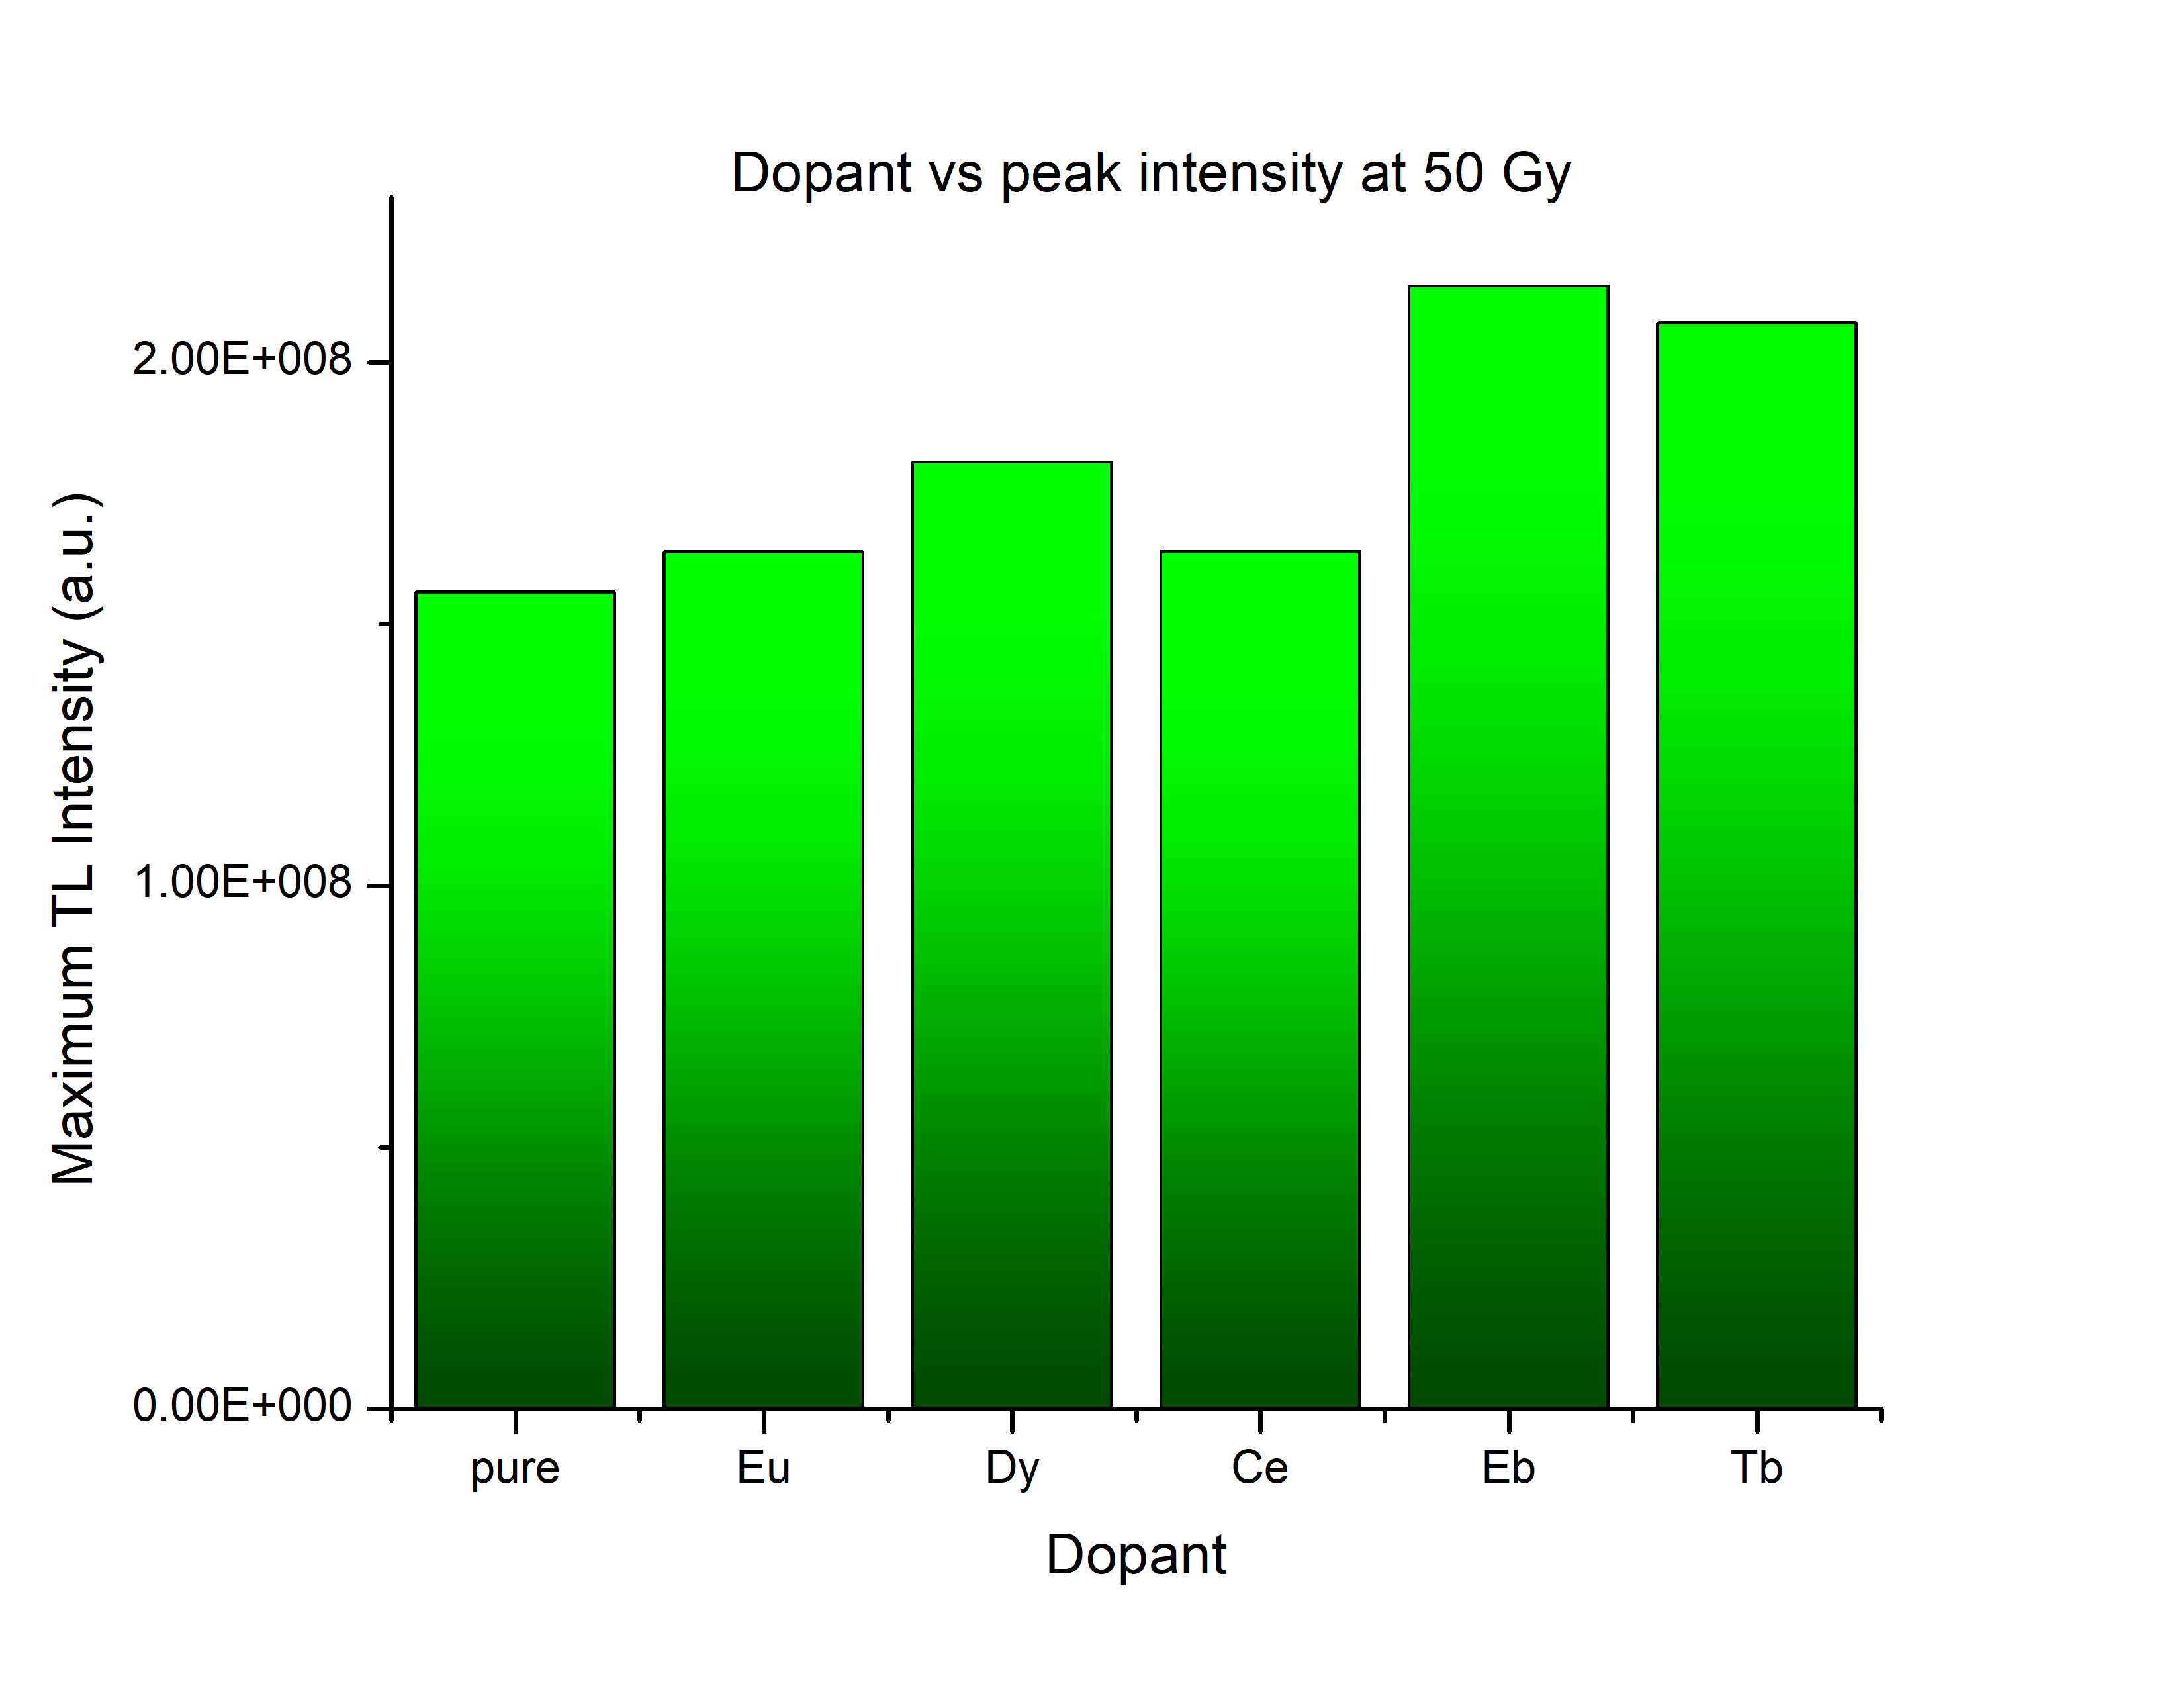
\includegraphics[width=0.6\linewidth]{intensity50.png}
            \captionof{figure}{Comparision of peak intensity for various dopants when irradiated with Gamma rays at 
            50 Gy}\label{fig:intensity50}
        \end{Figure}
        \begin{Figure}
            \centering
            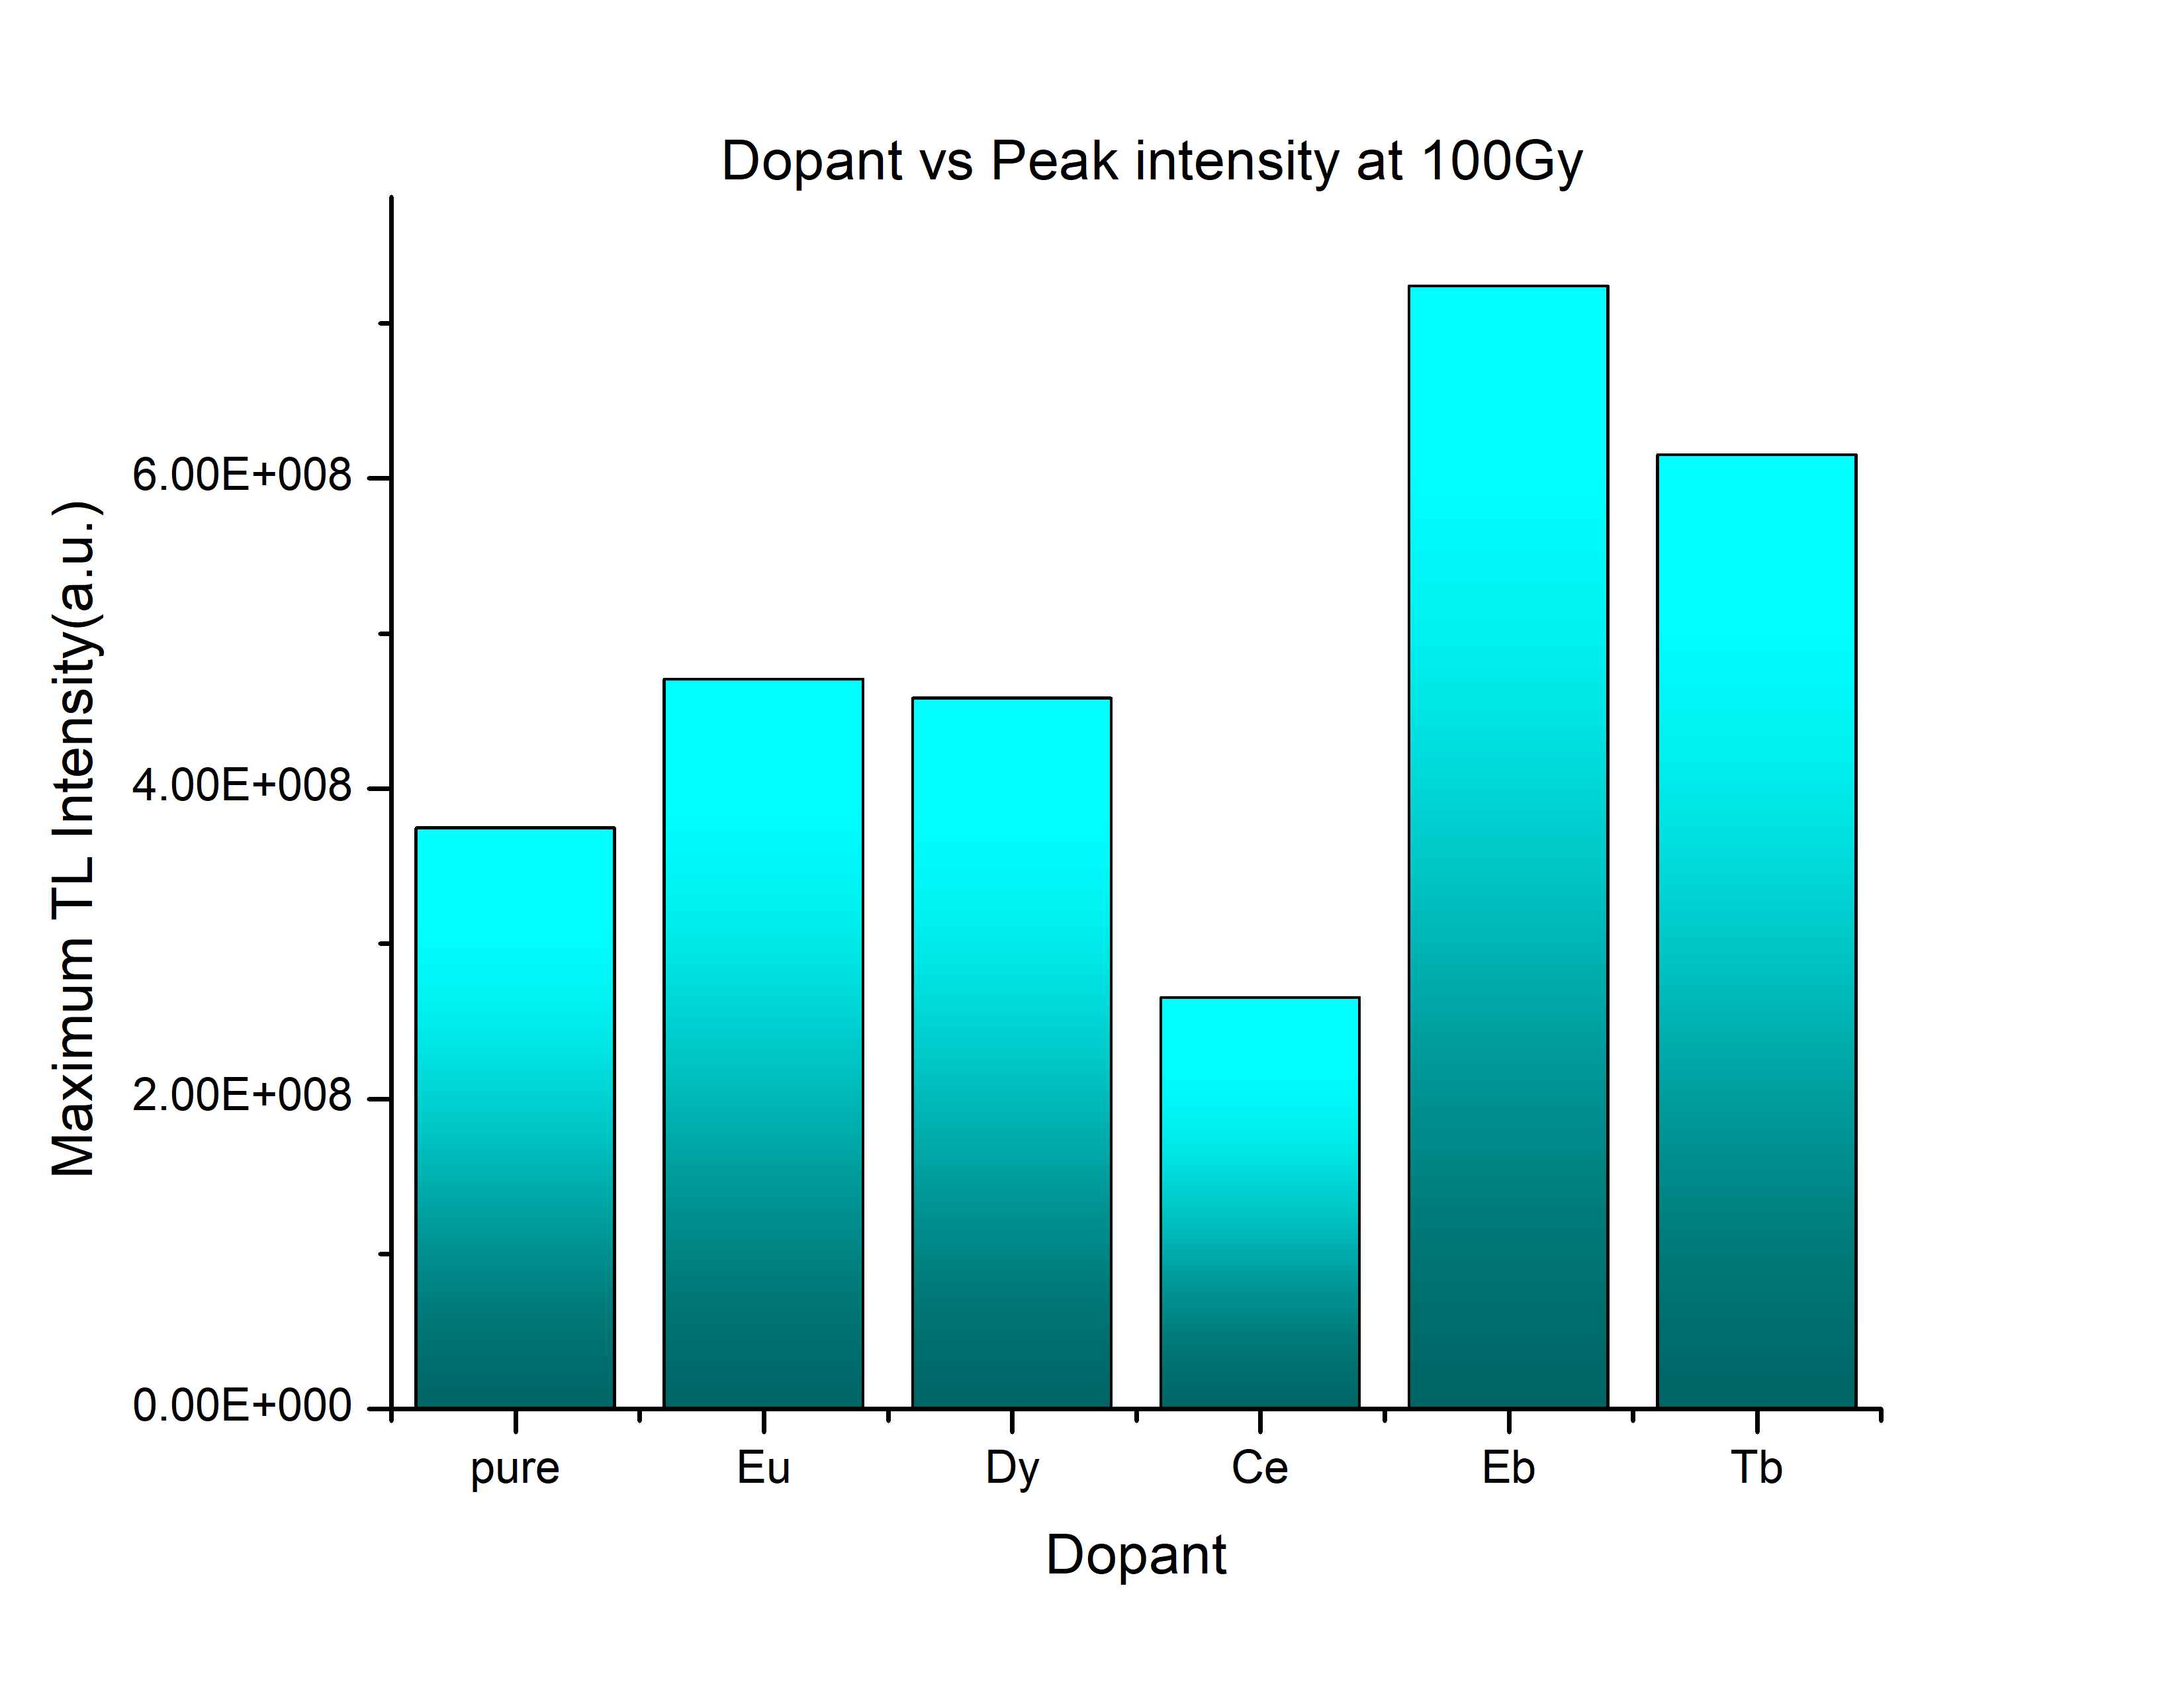
\includegraphics[width=0.6\linewidth]{intensity100.png}
            \captionof{figure}{Comparision of peak intensity for various dopants when irradiated with Gamma rays at 
            100 Gy}\label{fig:intensity100}
        \end{Figure}
    \end{multicols}

    Finally, it can be concluded that lithium metasilicate shows thermoluminescence and yields distinct peaks for definite
    temperatures with maximum intensity at higher temperatures. On addition of dopants, the thermoluminescence intensities in
    much higher than that of undoped sample. Doping with Terbium and Erbium results in maximum intensities for 50 Gy and 100 Gy 
    gammma irradiation. More analysis is required in this field to provide a conclusive evidence of the use of lithium metasilicate
    as a viable and effective material for thermoluminescence dosimetry.
\end{document}